\documentclass{report}
\usepackage[a4paper, total={6in, 8in}]{geometry}
\usepackage[style=numeric,backend=biber]{biblatex}
\usepackage[italian]{babel}
\usepackage[utf8]{inputenc}
\usepackage{newlfont}
\usepackage{hyperref}
\usepackage{graphicx}
\usepackage{placeins}
\usepackage{minted}
\usepackage{url}
\usepackage{subfig}
\usepackage{float}
\usepackage{afterpage}
\usepackage{todonotes}
\addbibresource{tesi.bib}
\usepackage{csquotes}

\hypersetup{
    colorlinks,
    citecolor=black,
    filecolor=black,
    linkcolor=black,
    urlcolor=black
}

\newcommand\myemptypage{
    \null
    \thispagestyle{empty}
    \newpage
}
    
\textwidth=450pt\oddsidemargin=0pt
\begin{document}
\begin{titlepage}
\begin{center}
{{\Large{\textsc{Alma Mater Studiorum $\cdot$ Universit\`a di
Bologna}}}} \rule[0.1cm]{15.8cm}{0.1mm}
\rule[0.5cm]{15.8cm}{0.6mm}
{\small{\bf SCUOLA DI INGEGNERIA E ARCHITETTURA\\
Corso di Laurea in Ingegneria Informatica }}
\end{center}
\vspace{15mm}
\begin{center}
{\LARGE{\bf Analisi delle performance}}\\
\vspace{3mm}
{\LARGE{\bf di Data-Plane Development Kit}}\\
\vspace{3mm}
{\LARGE{\bf in dispositivi virtualizzati P4 }}\\
\end{center}
\vspace{40mm}
\par
\noindent
\begin{minipage}[t]{0.47\textwidth}
{\large{\bf Relatore:\\
Chiar.mo Prof.\\
Marco Prandini}}
\vspace{1cm}
\end{minipage}
\\
\begin{minipage}[t]{0.47\textwidth}
{\large{\bf Correlatori:\\
Dott. Amir Al Sadi\\
Dott. Andrea Giovine}}

\end{minipage}
\hfill
\begin{minipage}[t]{0.47\textwidth}\raggedleft
{\large{\bf Presentata da:\\
Patrick Di Fazio}}
\end{minipage}
\vspace{20mm}
\begin{center}
{\large{\bf Sessione 1\\
Anno Accademico 2021-2022}}
\end{center}
\end{titlepage}



\myemptypage

\tableofcontents
\newpage

\chapter*{Abstract}
\addcontentsline{toc}{chapter}{Abstract}


Data Plane Development Kit è un set di librerie a basso livello, scritto in linguaggio C, che offre elevate prestazioni a livello di Data Plane, una branca del Software Defined Networking che si occupa di forwarding e che offre numerosi vantaggi sfruttando la tecnologia del Kernel Bypassing. 
Per analizzare le prestazioni di DPDK sono stati usati dei generatori di traffico collegati a degli switch programmati con Programming Protocol-Indipendent Packet Processors (P4), un linguaggio di programmazione utilizzato per configurare regole e azioni dei dispositivi di rete.
Si presenta di seguito l'analisi delle prestazioni con utilizzo della tecnologia P4, che prevede l'impiego di uno o più switch interposti tra un ricevente e il generatore di traffico DPDK. Lo studio è condotto tenendo conto della quantità di pacchetti che vengono persi durante l'inoltro, della velocità effettiva di inoltro e della potenza di calcolo richiesta per effettuare la trasmissione.
I risultati suggeriscono una elevata capacità di generazione di pacchetti sfruttando DPDK e mettono in risalto la riprogrammabilità degli switch P4.
Diverse infrastrutture generano diversi risultati, con prestazioni variabili.
L'analisi dei risultati è utile in funzione ai possibili sviluppi futuri. Unendo le prestazioni di DPDK alla versatilità di P4, sarebbe possibile avanzare un nuovo approccio alle SDN migliorandone le performance a livello Data Plane.
\newpage
\newpage
\myemptypage
\chapter*{Capitolo 1}
\addcontentsline{toc}{chapter}{Capitolo 1}

\section*{Introduzione}
\addcontentsline{toc}{section}{Introduzione}


Le reti moderne distaccandosi dal classico modello di rete chiusa, possono adottare nuovi sviluppi e innovazioni come quelli introdotti dalle SDN.
P4 si propone come linguaggio con un grande potenziale. Grazie alla sua programmabilità, permette infatti di rendere le funzioni che una volta erano cablate nel firmware del dispositivo, aperte, programmabili e modificabili a runtime. L'approccio adottato è infatti quello ``top-down", dove è il programmatore che definisce le funzionalità che la rete deve avere, senza essere limitato dall'hardware che il vendor produce, tipico scenario dell' approccio ``bottom-up" delle reti tradizionali.
Questo consente di allontanarsi dal modello in cui la rete è sviluppata, sfruttando la sinergia tra hardware e software, e di centralizzare lo sviluppo del networking sulla base di programmi scritti dallo sviluppatore che ora è in grado di avere una completa panoramica sulle funzionalità dell'ambiente in cui opera.\\
DPDK fornisce delle migliorie a livello di Data Plane. Grazie alle sue librerie ottimizzate, riesce a velocizzare il forwarding dei pacchetti sfruttando tecnologie come il Kernel Bypassing, che verranno approfondite in seguito. DPDK riesce infatti a portare nello user-space e quindi a livello utente, le interfacce di rete che prima erano legate al Kernel, delegando alla NIC (Network Interface Controller) il completo controllo dell'applicazione.\\
Questo paradigma permette di avere una visione completamente nuova della rete. Coniugando queste due tecnologie sarebbe possibile infatti controllare l'instradamento di pacchetti accelerandone le prestazioni, senza essere legati all'hardware del dispositivo.

\newpage


\section*{Software Defined Networks}
\addcontentsline{toc}{section}{Software Defined Network}
Con le SDN si disaccoppiano hardware e software, rendendo disponibile una ampia programmabilità di rete che permette di sfruttare anche più nodi, caricare regole dinamicamente e su richiesta dell'amministratore di rete senza avere notevoli perdite di pacchetti. Grazie alla virtualizzazione della rete si possono caricare infatti le regole ``on the fly'', permettendo di cambiare le configurazioni degli switch e dei router mentre sono accesi, con una perdita di pacchetti quasi nulla.
Nelle reti Software Defined si disaccoppiano anche il livello di inoltro dei pacchetti, il cosiddetto Forwarding Plane o Data Plane, dal modello di Control Plane, che si occupa di come i pacchetti vengono inoltrati.
Si realizza così una netta divisione che permette lo sviluppo di tecnologie separate per livelli separati, rendendo la rete completamente aperta dal punto di vista del programmatore.\\
Grazie alla loro flessibilità e dinamicità e grazie alla loro predisposizione ad una rete divisa su più nodi, le SDN hanno trovato luogo nel Cloud Computing, dove è necessario gestire una grande quantità di dati. Restano però ancora aperti i numerosi problemi di sicurezza che un approccio così centralizzato può avere. In {\textbf{Figura \ref{fig:sdn}}} è mostrata l'architettura di una SDN, in particolare i due livelli di Data e Control Plane. \cite{noauthor_software_nodate}
\vspace{1cm}
\FloatBarrier
\begin{figure}[!htbp] 
    \centering
    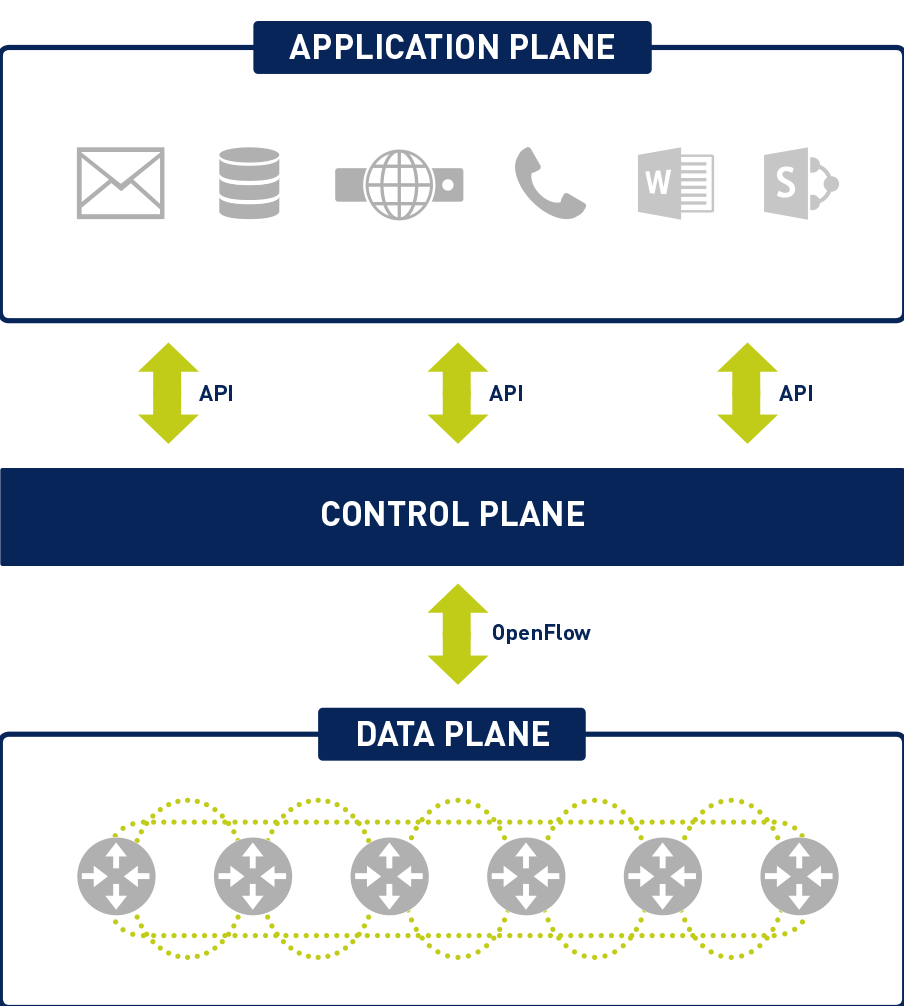
\includegraphics[scale=0.32]{images/sdn.png}
    \caption{\textit{Architettura delle SDN}}
    \label{fig:sdn}
\end{figure}
\FloatBarrier

\subsection*{Control Plane}
\addcontentsline{toc}{subsection}{Control Plane}

Il Control Plane è il piano di controllo adibito a numerosi ruoli.
Nelle SDN che utilizzano OpenFlow \cite{noauthor_openflow}, il Control Plane si occupa della scelta del percorso del pacchetto in rete, della popolazione della Routing Table e della Forwarding Table.
Le nuove reti SDN, invece, puntano alla riprogrammabilità a livello di Data Plane, delegando a questo livello le decisioni sull'instradamento dei pacchetti. P4, ad esempio, riesce a rendere programmabili i dispositivi come gli switch iniettando direttamente le regole per il forwarding e definendo tramite il ``codice P4", che verrà compilato in un eseguibile, le azioni che il dispositivo deve svolgere.\\

\subsection*{Data Plane}
\addcontentsline{toc}{subsection}{Data Plane}
Il Data Plane è la parte effettiva che si occupa del forwarding dei pacchetti. È il livello che si occupa del controllo del flusso reale dei dati che passano in rete.
Generalmente, dopo aver ricevuto direttiva di inoltro da parte del piano di controllo, si applica il forwarding ai pacchetti. A questo livello è fondamentale per la velocità della rete avere degli algoritmi efficaci tali che usino meno risorse possibili. È in questo piano che poniamo DPDK e P4.

\subsection*{Tecnologie Utilizzate e Casi D'Uso}
\addcontentsline{toc}{subsection}{Tecnologie Utilizzate e Casi D'Uso}
Di seguito sono elencate alcune delle tecnologie a livello applicativo nelle quali è possibile introdurre le SDN, in particolare P4 e DPDK. 

\begin{itemize}
    \item \textbf{Indipendenza dai Protocolli}. Le SDN forniscono una programmabilità versatile che permette di specificare il parsing degli header dei pacchetti di dati (anche a runtime), rendendo i programmi, come quelli su switch P4, adattabili al tipo di protocollo adottato.
    \item \textbf{Monitoraggio di Rete}. Fornendo un Data Plane programmabile, con P4 è possibile monitorare e analizzare il traffico di rete introducendo specifiche regole e azioni da applicare con l'arrivo di determinati header o pacchetti di dati. Un esempio reale è l'introduzione di una DoS protection tramite le SDN \cite{navid_detection_2017}.
    \item \textbf{Distribuzione della Rete}. Con le SDN in generale, ma nello specifico con P4, è possibile costruire una rete virtuale composta da molti nodi, centralizzata e programmabile ``on the fly" che permette di applicare modifiche molto velocemente. Uno caso molto diffuso è quello delle Virtual Private Cloud (VPC) offerte da Amazon Web Services (AWS), ovvero reti virtuali interne che servono per isolare spazi di lavoro \cite{noauthor_aws_sdn}.
    \item \textbf{Controllo della Rete}. Tramite le SDN è possibile applicare ai dati in arrivo le politiche di Load Balancing, Congestion Control e Logging così da gestire la rete mantenendone il massimo controllo. Queste soluzioni possono essere adottate a livello Enterprise per avere un alto livello di ``Governance" sulle proprie reti interne. Un chiaro esempio di Load Balancing basato su SDN è il SLB (Software Load Balancer) di Microsoft Azure \cite{noauthor_azure_sdn}.
    \item \textbf{Velocità di trasmissione}. Con DPDK è possibile trasmettere dati ad una velocità elevata anche utilizzando hardware di basso costo, rendendo così le SDN adattabili a tecnologie di uso quotidiano. Un caso di utilizzo di DPDK a livello Server è nell'introduzione di questa tecnologia nei Data Center di Lenovo \cite{noauthor_lenovo_sdn}.
\end{itemize}






\newpage
\chapter*{Capitolo 2}
\addcontentsline{toc}{chapter}{Capitolo 2}

\section*{Tecnologie Utilizzate}
\addcontentsline{toc}{section}{Tecnologie Utilizzate}

\section*{Data-Plane Development Kit}
\addcontentsline{toc}{section}{Data-Plane Development Kit}

Data-Plane Development Kit è un framework sviluppato da Intel, con primo rilascio nel 2010 e ora supportato da The Linux Foundation. DPDK consiste in un set di librerie e di driver che consentono  di accelerare il packet processing.
Il suo punto di forza consiste nell'eseguire le applicazioni direttamente in user-space, in modo che vengano eseguite direttamente sulla NIC. 
Uno dei punti di forza di DPDK è la performance elevata su piccoli pacchetti di dati.
Un flusso di dati con pacchetti di piccole dimensioni (tipicamente 64 byte) viene gestito male dal Networking Stack di Linux perché genera un numero elevato di interrupt (uno per ogni pacchetto). Grazie ai Poll Mode Driver di cui fa uso DPDK, la gestione diventa a polling in modo da usare una minore quantità di interrupt.\\
DPDK sfrutta inoltre il Kernel Bypassig, così da non consultare il Networking Stack e avere prestazioni migliori.
Le applicazioni in questo modo riescono a dialogare direttamente con la NIC che riceve il traffico di dati, senza interferire con il Kernel.
DPDK è compatibile con un vasto numero di CPU, architetture e schede di rete. Gli obiettivi del set di librerie sono i seguenti.
\begin{itemize}
    \item Ricevere e inviare i pacchetti nel minor numero possibile di cicli della CPU, per massimizzare l'efficienza del Data Plane
    \item Catturare i pacchetti più velocemente possibile
    \item Essere compatibile con i Fast Path Stack di terze parti
\end{itemize} 
\pagebreak
In \textbf{Figura \ref{fig:helloworld_dpdk}} è presente l'esempio di un programma che stampa ``Hello World" con DPDK.
\FloatBarrier
\begin{figure}[h]
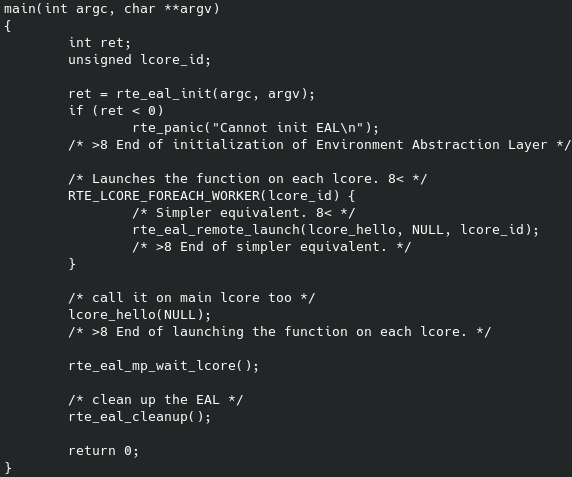
\includegraphics[width=7.5cm]{images/helloworld_dpdk.png}
\centering
\caption{\textit{Hello World con DPDK}}
\label{fig:helloworld_dpdk}
\end{figure}
\FloatBarrier
\section*{Kernel Bypassing}
\addcontentsline{toc}{section}{Kernel Bypassing}
DPDK adotta il Kernel Bypassing \cite{enberg_kernel-bypass_2018} e grazie a questo riesce a raggiungere prestazioni elevate.
Il Kernel Bypassing permette di saltare lo stack di networking che è presente nei sistemi operativi, ovvero i vari livelli che un pacchetto di rete deve percorrere per arrivare alla scheda di rete. La completa eliminazione del passaggio del pacchetto nello stack, è possibile grazie all' astrazione che DPDK introduce portando nello user-space le applicazioni. In questo modo il dialogo tra hardware e software non avviene più a livello del Kernel, ma viene portato sulla scheda di rete. Questo avvantaggia il processo di ricezione e invio del singolo dato perché soggetto ad una pipeline più breve e meno operazioni di copia. In \textbf{Figura \ref{fig:kernel_bypassing}} si mostra il livello di direttezza del Kernel Bypassing.

\FloatBarrier
\begin{figure}[h]
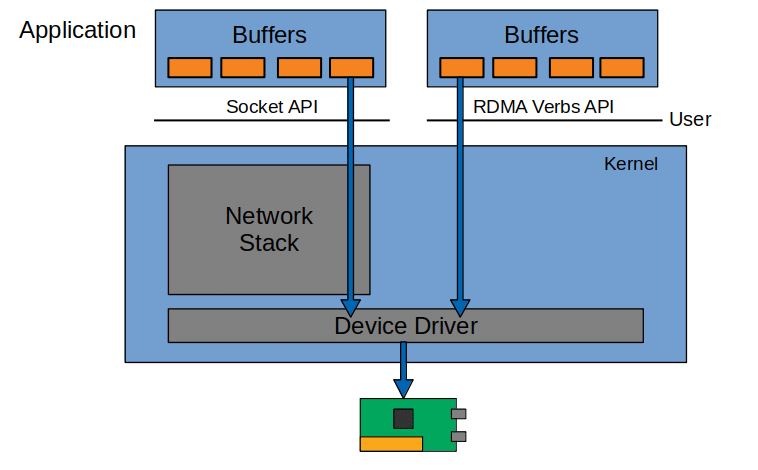
\includegraphics[width=8cm]{images/kernel_bypassing.png}
\centering
\caption{\textit{Accesso diretto alla NIC grazie al Kernel Bypassing}} \cite{noauthor_kernel-networking-vs-kernel-bypassingppm_nodate}
\label{fig:kernel_bypassing}
\end{figure}
\FloatBarrier

\subsection*{Vantaggi di DPDK}

\vspace{2mm}
\addcontentsline{toc}{subsection}{Polling}
\subsubsection*{Polling}
DPDK sfrutta i Poll Mode Drivers (PMD) ovvero una modalità a polling che si contrappone al classico modello ad interrupt e che è funzionale nel caso in cui si gestiscano enormi quantità di dati (esempio reti da \textbf{1 - 2 Gbit/s}).\\
Questa modalità prevede che assegnando, ad esempio, i core 1 e 2 (flag -l 0-1) su 4 core di sistema, i primi due core verranno dedicati interamente alla gestione del polling di DPDK. Questo succede perché vengono considerati in modalità non-preemptive e prioritaria: ogni volta che viene richiesto un pacchetto, i due core hanno la priorità di esecuzione sulla gestione di questo.
I pacchetti sono gestiti in code (queues) e la CPU li può leggere in base al carico  dati che ha in quel momento.\\
La CPU notifica la NIC nel momento in cui è possibile leggere altre code e così la NIC può inviare nuovamente l'interrupt per i prossimi dati.

\vspace{2mm}
\addcontentsline{toc}{subsection}{Zero Copy}
\subsubsection*{Zero Copy}
Nel corso dell' arrivo di un pacchetto e del successivo processamento, una nuova copia viene generata all'interno dell'applicazione che lo ha richiesto. Con DPDK, avendo la NIC il diretto accesso ai pacchetti, si dimezza il tempo necessario in quanto le librerie di cui fa uso consentono di impiegare direttamente i dati in arrivo, in modo ``raw" (la NIC ne prende totalmente carico), senza doverli copiare.

\vspace{2mm}
\addcontentsline{toc}{subsection}{User Defined Ring Buffer}
\subsubsection*{User Defined Ring Buffer}
DPDK delega completamente e in modo trasparente alla NIC la gestione del pacchetto e quindi il Kernel non attiva nessun ring.
\leavevmode\newline
In \textbf{Figura \ref{fig:dpdkdifferences}} sono presentate le differenze tra un sistema che usa DPDK e un sistema che non lo usa.
\FloatBarrier
\vspace{1cm}
\begin{figure}[h]
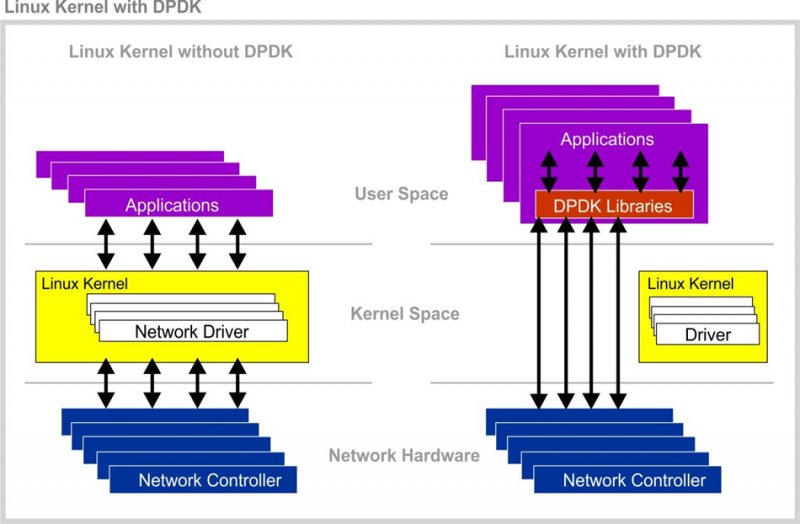
\includegraphics[scale=0.30]{images/dpdkdifferences.png}
\centering
\caption{\textit{Vantaggi di DPDK}}
\label{fig:dpdkdifferences}
\end{figure}
\FloatBarrier

\addcontentsline{toc}{section}{DPDK nel dettaglio}
\subsubsection*{DPDK nel dettaglio}
Il set di librerie che DPDK offre è diviso in molti punti chiave. Riassumendo, il ``core" del framework è suddiviso nei seguenti componenti.
\begin{itemize}
    \item \textbf{Memory Manager} responsabile dell' allocazione di pool di oggetti in memoria
    \item \textbf{Buffer Manager} prealloca la memoria necessaria pronta per l'uso all'esecuzione di DPDK
    \item \textbf{Queue Manager} implementa le code utilizzabili se supportate dalla scheda di rete, sia per la ricezione che per la trasmissione
    \item \textbf{Flow Classification} permette di introdurre i pacchetti più velocemente nel flusso di dati
    \item \textbf{Poll Mode Drivers} evita di usare il meccanismo classico ad interrupt. Dei core della CPU si dedicano completamente al polling rendendo la CPU sempre disponibile alla ricezione o all'invio di pacchetti.
\end{itemize}

\addcontentsline{toc}{subsection}{Hugepages}
\subsection*{Hugepages}
Le Hugepages sono blocchi di memoria di dimensione variabile, composti da singole pagine da 4096 byte. DPDK utilizza le ``Persistent Hugepages" allocate in modo dinamico, più stabili delle tipiche ``Transparent Hugepages" che sono allocate a runtime in modo automatico.\\
Usando pagine di grande dimensione è possibile accedere alla memoria più velocemente. Queste sono infatti preallocate per l'esecuzione del programma e permettono di migliorare le performance del sistema, non dovendo allocare memoria per ogni operazione richiesta. 
Secondo la documentazione di DPDK è consigliato usare Hugepages da 1GB, ovvero preallocare 256.000 pagine di memoria.\\
Conseguentemente al grande numero di pacchetti che si deve gestire, essendo DPDK pensato per gestire flusso dati su larga scala, si utilizzano le hugepages per evitare di accedere al disco per ogni pacchetto in arrivo. La memoria è preallocata e non ha bisogno di essere riallocata per ogni operazione di rete: si evitano molti problemi e si garantisce velocità di lettura.
Usando normali pagine si avrebbero molte più entry da controllare, ciò risulterebbe in un maggiore ``tempo di burst" per la CPU.\\
Le hugepages possono essere da 2M o da 1GB. Nel caso di una Virtual Machine si possono usare 2048K di pagine per far funzionare correttamente la suite DPDK. Per lo studio delle prestazioni in trasmissione e ricezione sono state usate delle pagine da 1GB all' interno di una macchina virtuale.

\addcontentsline{toc}{subsection}{Environment Abstraction Layer (EAL)}
\subsection*{Environment Abstraction Layer (EAL)}
L' Environment Abstraction Layer è il responsabile dell'accesso alle risorse a basso livello e alla memoria. È un livello generico di astrazione che permette di eseguire DPDK senza che esso conosca l'hardware sottostante. I compiti dell' EAL sono molteplici, come ad esempio avviare DPDK, assegnare le istruzioni agli specifici core e riservare zone di memoria per le interazioni con la scheda di rete.\\
Per il setup, il programma ha bisogno della funzione \textbf{rte\_eal\_init()} che inizializza l' Enviroment Abstraction Layer in modo da accedere alle risorse di basso livello. In particolare utilizzando le librerie \textbf{pthread} possiamo delegare ogni esecuzione ad un thread diverso (ad esempio in una macchina con 4 core che dispone di hyperthreading ad 8 thread, si può lanciare il programma delegando a tutti gli 8 core i vari processi).
L'inizializzazione come ogni programma \textbf{C} è delegata alla glibc, ma l'inizializzazione effettiva è una chiamata alle librerie phread eseguita tramite rte\_eal\_init().
Al termine del programma, per la deallocazione delle risorse si ha una chiamata a \textbf{rte\_eal\_cleanup()}
In \textbf{{Figura \ref{fig:EAL}}} è mostrata l'inizializzazione delle EAL al lancio del programma con la conseguente creazione dei pthread. È quindi intuibile da questo tipo di startup che il programma sia stato eseguito su due core e quindi utilizzando gli specifici parametri EAL \begin{minted}[escapeinside=||]{py}
./program |\colorbox{lightgray}{-l 2}|
\end{minted}
\FloatBarrier
\begin{figure}[h]
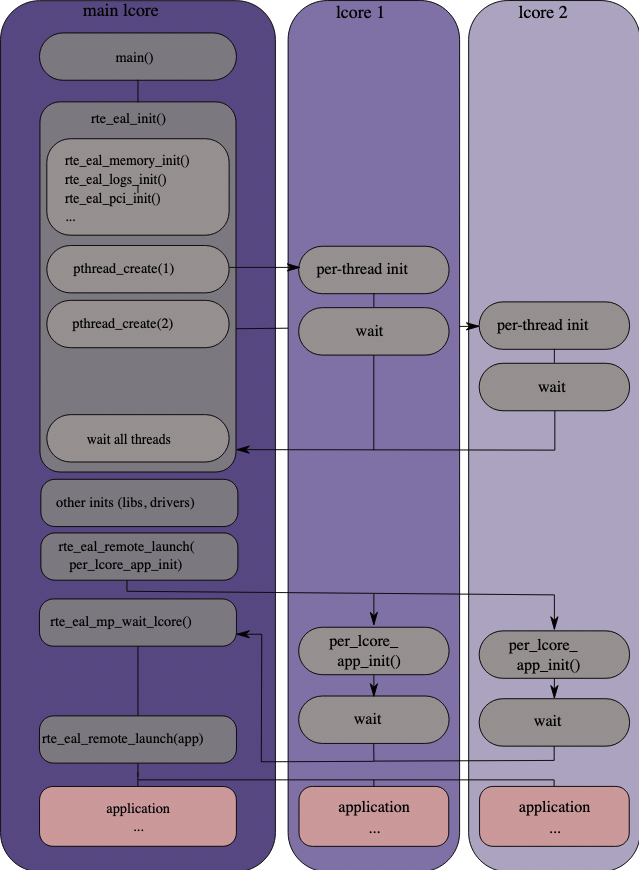
\includegraphics[scale=0.40]{images/EAL.png}
\centering
\caption{\textit{Inizializzazione dell' EAL}}
\label{fig:EAL}
\end{figure}
\FloatBarrier
\addcontentsline{toc}{subsection}{Poll Mode Drivers (PMD)}
\subsection*{Poll Mode Drivers (PMD)}
I Poll Mode Driver sono un set di API che hanno accesso ai canali di comunicazione in ricezione e trasmissione senza la necessità di utilizzare interrupt. Hanno la funzionalità di configurare i devices e le loro code e funzionano completamente nello user-space. Hanno il compito di processare e inviare i pacchetti nel modo più ottimizzato possibile e in base alle condizioni di carico del sistema al momento e sono configurabili ``on the fly".

\pagebreak
\addcontentsline{toc}{section}{Programming Protocol-Indipendent Packet Processors: P4}
\section*{Programming Protocol-Indipendent Packet Processors: P4}

P4 è un linguaggio di programmazione ad alto livello che abbraccia completamente il concetto di SDN, essendo ``Protocol Indipendent" \cite{noauthor_p4_nodate}. Permette allo sviluppatore di implementare uno Networking Stack personale in hardware di rete come switch o router. La forza di P4 è dare al programmatore tutti gli strumenti necessari per programmare dispositivi di switching in modo da essere facilmente configurabili sulla base di esigenze sempre nuove, come l'introduzione di nuovi header. Grazie alla sua versatiltà può essere introdotto in router, switch o altri dispositivi di rete che processano pacchetti. P4 può essere applicato e  compilato per un grande numero di dispositivi che vengono chiamati ``Targets". Per ogni dispositivo su cui agisce P4, possono essere predisposte diverse regole.

\addcontentsline{toc}{subsection}{Architettura}
\subsubsection*{Architettura}
L'architettura PSA (Portable Switch Architecture) \cite{noauthor_p4_2022} descrive le caratteristiche principali che hanno dispositivi di rete come switch, per processare ed inoltrare pacchetti. PSA contiene la libreria di tipi e costrutti disponibili per programmi P4 standard.
Il modello PSA ha sei ``Programmable Blocks" e due ``Fixed Function Blocks". I blocchi sono programmabili tramite P4, mentre i restanti due blocchi dipendono dal target sul quale sono applicati. In \textbf{{Figura \ref{fig:pipeline_p4}}}
 si vede la classica pipeline di una PSA.
\vspace{1cm}
\begin{figure}[h]
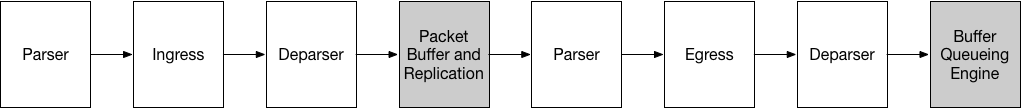
\includegraphics[scale=0.4]{images/pipeline_p4.png}
\centering
\caption{\textit{PSA Pipeline}}
\label{fig:pipeline_p4}
\end{figure}
\leavevmode\newline
Con questa pipeline si validano i pacchetti in arrivo al dispositivo di rete e si applicano le regole che sono stabilite su ingress (match + action). Il primo Function Block permette all'evenienza di duplicare i pacchetti per funzionalità future. Alla fine della pipeline il pacchetto viene serializzato e spedito dal secondo Function Block ai successivi riceventi.
\addcontentsline{toc}{subsection}{Header}
\subsubsection*{Header}
P4 può supportare una gamma di protocolli così vasta grazie alla riconfigurabilità che hanno i suoi header. Gli header di un pacchetto P4 infatti possono essere definiti in modo personalizzato così che si possano adattare all'esigenza della rete, in modo che all'aggiunta in rete di nuovi protocolli, il programma P4 si possa adattare ai nuovi pacchetti. La sintassi degli header è simile a quella delle strutture in C.

\addcontentsline{toc}{subsection}{Parser e Deparser}
\subsubsection*{Parser e Deparser}
Un programma P4 deve essere disposto di un parser e di un deparser \cite{noauthor_notitle_nodate}. Il parser serve a collegare la rappresentazione a bit del pacchetto alla reale struttura dati che lo rappresenta nel linguaggio P4: i dati vengono inseriti in un pacchetto su cui viene eseguito il parsing.
Il deparser ha invece il compito di ricostruire il flusso di bit che verrà ritrasmesso in rete, serializzando l'header e i vari campi che compongono il pacchetto. Dato che nei programmi P4 possono essere introdotti anche nuovi header, è necessario che il parser ed il deparser conoscano la struttura dei pacchetti di rete sui quali vanno ad operare.
Il codice sottostante mostra il parsing di header ethernet e IPv4.

\begin{minted}
[
frame=lines,
framesep=2mm,
baselinestretch=1.2,
bgcolor=white,
fontsize=\footnotesize,
linenos
]
{c}
state start {
return parse_ethernet;
}
state parse_ethernet {
  packet.extract(headers.ethernet);
  return select(headers.ethernet.etherType) {
    0x800 : parse_ipv4;
    default : accept;
  }
}
state parse_ipv4 {
  packet.extract(headers.ipv4);
  return accept;
}   
\end{minted}

\addcontentsline{toc}{subsection}{BMv2 Target}
\subsection*{BMv2 Target}
Uno dei target disponibili su cui lanciare P4 è il behavioral-model 2 che si propone come modello di test, con prestazioni non troppo elevate, ma utile al fine di vedere nella pratica le regole applicate ai dispositivi di rete e utile per la fase di debug. 
Per incrementare le prestazioni di BMv2, è possibile compilare il target con delle flag specifiche \cite{noauthor_behavioral_2022}.
\begin{minted}{bash}
./configure 'CXXFLAGS=-g -O3' 'CFLAGS=-g -O3' 
--disable-logging-macros --disable-elogger
\end{minted}
La suite di BMv2 predispone anche un benchmark per il testing delle prestazioni. Alla fine del tuning si dovrebbero raggiungere le prestazioni di circa 1Gbit/s, molto più elevate rispetto a quelle in assenza di tuning (che si aggirano attorno ai 300 Mbit/s). 

\section*{Tecnologie di Virtualizzazione}
Nelle sezioni successive sono riportate le tecnologie utilizzate durante la fase di progetto inerenti alla virtualizzazione e al setup dell' Hypervisor.

\addcontentsline{toc}{section}{Tecnologie di Virtualizzazione}

\subsection*{Interfacce TUN/TAP}
\addcontentsline{toc}{subsection}{Interfacce Tun/Tap}
TUN e TAP sono driver che hanno la funzionalità di creare periferiche virtuali di rete \cite{noauthor_universal_nodate}. Queste interfacce virtuali permettono di simulare le connessioni fisiche al sistema, agendo come se fisicamente connesse alla scheda di rete dell'host.\\
Le interfacce TAP lavorano a livello data-link e quindi a livello 2 dello stack ISO/OSI, mentre le interfacce TUN agiscono da connessione punto a punto e si collocano a livello 3. 
Sono fisicamente accessibili da /dev/net/tun.
Nei setup successivi, il device driver utilizzato sarà MacVTap \cite{noauthor_using_nodate}, ovvero una versione semplificata che rimpiazza la combinazione Tun/Tap e supportato da QEMU/KVM \cite{noauthor_qemu_nodate} \cite{principles}.

\subsection*{Namespace}
\addcontentsline{toc}{subsection}{Namespace}
I namespace sono spazi di nomi che rinchiudono risorse al loro interno, facendo apparire i processi come separati dal resto del sistema. Sono essenzialmente una astrazione che il sistema operativo fa per far apparire processi separati come risorse separate. Su Linux un processo di un namespace esistente si trova sotto la cartella \textbf{$/proc/<pid>/ns$}.
Durante l'attività di progetto è stato utile creare namespace per fare dei test tra ambienti separati, come se la comunicazione avvenisse tra calcolatori diversi. Per far comunicare i namespace a ognuno è stato assegnato un IP e sono stati collegati tra loro tramite Virtual Ethernet Device.\\
I namespaces vengono creati con i seguenti comandi
\begin{minted}{bash}
ip netns add net1
ip netns add net2
\end{minted}
\subsection*{Virtual Ethernet Device (Veth)}
\addcontentsline{toc}{subsection}{Virtual Ethernet Device}
Sono dispositivi di rete virtuali che agiscono da tunnel collegando namespaces. Le veth \cite{noauthor_veth} hanno la funzione di bridge o cavo e sono create sempre a coppie. Nella fase di progetto sono state utilizzare per connettere due namespaces su cui risiedevano gli host H1 e H2 collegati agli switch.
mentre la coppia di veth viene creata in questo modo
\begin{minted}{bash}
ip link add veth1 netns net1 type veth peer name veth2 netns net2
\end{minted}
\section*{Altre Tecnologie}
\addcontentsline{toc}{section}{Altre Tecnologie}
Di seguito sono riportate alcune delle tecnologie legate a DPDK e alle SDN non analizzate in questa tesi.
\addcontentsline{toc}{subsection}{OpenVSwitch}
\subsection*{OpenVSwitch}
OpenVSwitch è un' implementazione software di uno switch a più livelli, ovvero offre tutte le funzionalità di uno switch ma può agire, se configurato, anche a livelli OSI superiori. Ha l'obiettivo di rendere programmabile la rete a livello switching. Può essere portato direttamente nello user-space ed è configurabile per sfruttare la tecnologia DPDK a livello Data Plane.\\


\addcontentsline{toc}{subsection}{Vector Packet Processing}
\subsection*{Vector Packet Processing}
VPP, Vector Packet Processing, è un Network Stack ad alte prestazioni, scalabile e che esegue direttamente nello user-space.
Fa parte del progetto FD.io di The Linux Foundation e usa un framework che può offrire varie funzionalità di rete come switching e routing \cite{noauthor_what_nodate}.
VPP può essere utilizzato negli switch e router virtuali, in Firewall e altro ancora.
Il vantaggio di VPP è dato dall'abbandono del classico modello di processamento scalare dei pacchetti. Nel modello classico infatti i pacchetti che arrivano al Kernel sono processati uno alla volta in seguito all'arrivo di un interrupt per pacchetto.
Con il modello vettoriale, è possibile processare i pacchetti secondo un vettore. Così facendo si ha la notifica dell'arrivo del vettore da un solo interrupt. Il vettore di pacchetti è poi prelevato dalla scheda di rete e processato secondo un set di funzioni.
La pipeline di ricezione si riassume nel ``Packet Processing Graph" \cite{noauthor_packet_nodate} presentato nella \textbf{{Figura \ref{fig:vpp_graph}}}
.\\
VPP alimenta un ring di ricezione di dati fino ad un massimo di 256 pacchetti, il grafo ricostruisce poi tutto l'albero di arrivo dei pacchetti e li processa.
Le prestazioni di questa tecnologia sono massimali quando il vettore di ricezione è di dimensione maggiore, dato che con una sola lettura si processano più pacchetti.
VPP è in grado di implementare vari plugin, come ad esempio il plugin che sfrutta MEMIF \cite{noauthor_fdio_nodate} o quello che usa DPDK.
\FloatBarrier
\begin{figure}[h]
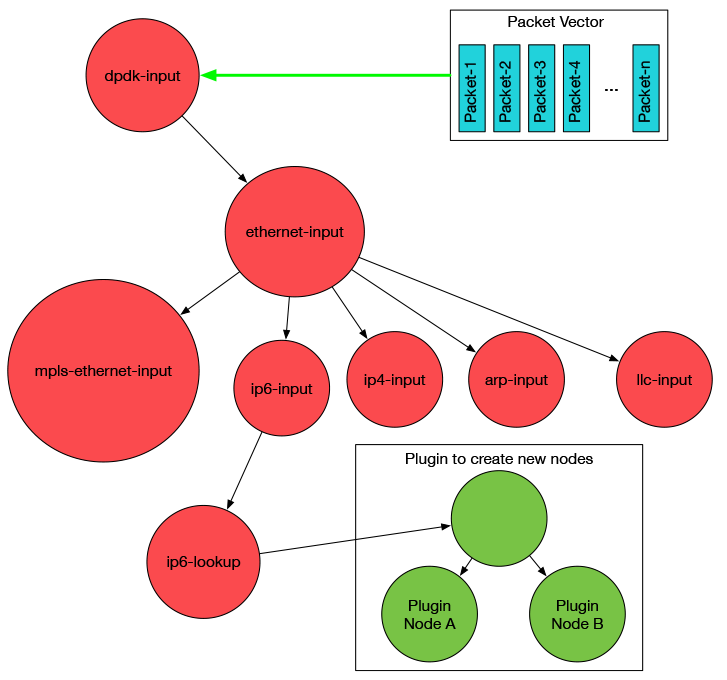
\includegraphics[scale=0.4]{images/vpp_graph.jpg}
\centering
\caption{\textit{OVS e OVS with DPDK}}
\vspace{1cm}
\label{fig:vpp_graph}
\end{figure}
\FloatBarrier

\addcontentsline{toc}{subsection}{VPP con plugin DPDK}
\subsection*{VPP con plugin DPDK}
Come si nota in \textbf{{Figura \ref{fig:vpp_graph}}}, è presente un elemento denominato \textit{dpdk-input}. Questo componente è un plugin caricato a runtime da VPP. Per abilitare il supporto a DPDK è inoltre necessario eseguire un ``binding" tra la scheda di rete e i driver DPDK. Andando a modificare il file di configurazione di VPP, un esempio chiaro di supporto ai driver DPDK può essere il seguente
\begin{minted}
[
frame=lines,
framesep=2mm,
baselinestretch=1.2,
bgcolor=white,
fontsize=\footnotesize,
highlightlines={22},
linenos
]{bash}


unix {
    nodaemon
    cli-listen /run/vpp/cli-vpp1.sock
    full-coredump
}
api-trace {
    on
    nitems 500
}
dpdk {
socket-mem 1024,2048

dev 0000:02:00.0 {
    num-rx-desc 1024
    num-rx-queues 2
}
dev 0000:01:00.0 {
    num-rx-desc 2048
    num-rx-queues 4
}
}
plugins { plugin dpdk_plugin.so {enable}}
\end{minted}
\newline
La parte evidenziata mostra come i plugin non siano altro che ``shared libraries" caricate a runtime da VPP. Il tag ``dev" indica il PCI address della scheda di rete riservata a DPDK. In questa configurazione sono presenti due schede di rete che sfruttano DPDK con due configurazioni differenti per il numero di descriptor nel buffer di ricezione e per il numero di code.
\newpage
\chapter*{Capitolo 3}
\addcontentsline{toc}{chapter}{Capitolo 3}

\section*{Descrizione del progetto}
\addcontentsline{toc}{section}{Descrizione del progetto}
Nella parte progettuale sono state usate e analizzate le tecnologie DPDK e P4 sul piano dell'inoltro dati. Lo scopo del progetto è infatti quello di trovare un modo per velocizzare l'instradamento dei pacchetti su degli switch P4. Per studiare i possibili modi per migliorare l'instradamento, prima sono stati svolti dei test di trasmissione tra due host usando solo DPDK e successivamente tra due host utilizzando solo P4. Alla fine sono stati registrati i risultati e confrontati a livello numerico, per avere un paragone tra le performance delle due tecnologie a livello di forwarding.
\newline
\\
La parte di progetto di DPDK ha come scopo quello di analizzare le performance della suite di librerie DPDK, in ambiente virtualizzato e ``Bare Metal". Per la generazione e la ricezione di pacchetti è stato usato il tool Pktgen DPDK \cite{wiles_pktgen_2022}.
La dimensione dei pacchetti è per tutti i test di 1500 byte.
\newline
\\
La parte di progetto riguardante P4 ha lo scopo di studiare le prestazioni di ricezione dati degli switch P4, più precisamente sfruttando il target BMv2. I test si riferiscono a un host interno ad una macchina virtuale. Le interfacce sono collegate tramite delle Veth passando per uno o più switch P4.
Gli switch P4 hanno un programma che fa accept e forward dei pacchetti, mentre gli host sono collocati su due namespaces differenti.

\section*{Sviluppo del progetto: DPDK}
\addcontentsline{toc}{section}{Sviluppo del progetto: DPDK}

\subsection*{Setup}
\addcontentsline{toc}{subsection}{Setup}
Per avere un supporto ai Poll Mode Drivers, è necessario abilitare l'apposito Kernel driver.
VFIO-PCI è un Kernel driver che permette un accesso diretto al dispositivo grazie alle sue API. È consigliato per l'uso con DPDK perché supporta l' IOMMU \cite{noauthor_iommu}, elemento essenziale per la comunicazione delle CPU con le periferiche, e può sfruttare il PCI Passthrough \cite{noauthor_pci_passthrough}, ovvero può collegarsi direttamente al dispositivo fisico PCI, rendendo le prestazioni ancora migliori.
Se si è impossibilitati ad abilitare VFIO, si può comunque usare il modulo standard \textbf{uio\_pci\_generic} incluso nel Kernel Linux, che però presenta qualche limitazione, poiché non supporta la creazione di funzioni virtuali.
È inoltre possibile fare il setup delle hugepages e successivamente disattivare la scheda di rete per renderla disponibile all'utilizzo. La NIC viene virtualmente separata dal device driver per essere associata a DPDK.\\ Il valore \textbf{02:00.0} corrisponde al PCI address della scheda di rete \cite{noauthor_6_nodate}.
I comandi con prefisso ``dpdk" fanno parte della suite fornita con l'applicativo. Per elencare le schede disponibili è possibile utilizzare
\begin{minted}{bash}
sudo dpdk-devbind.py -s
\end{minted}
Oppure manualmente con:
\begin{minted}{bash}
sudo lshw -c network -businfo
\end{minted}
Per velocizzare il setup si possono utilizzare le varie utility fornite dalla suite DPDK per montare le hugepages o fare il binding della scheda di rete.
La configurazione sottostante è la stessa per ogni host su cui eseguiranno le istanze di Pktgen.
\begin{minted}
[frame=lines,
framesep=2mm,
baselinestretch=1.2,
bgcolor=white,
fontsize=\footnotesize,
linenos
]{bash}
#!/bin/bash
modprobe uio
modprobe uio_pci_generic
dpdk-hugepages.py -p 1G --setup 2G
ifconfig enp2s0 down
dpdk-devbind.py -b uio_pci_generic 02:00.0
\end{minted}

\subsection*{Pktgen DPDK}
\addcontentsline{toc}{subsection}{Pktgen DPDK}
DPDK Pktgen è un generatore di traffico che sfrutta DPDK a livello Data Plane che permette di creare pacchetti personalizzati di dimensione, IP/MAC source/destination, arbitrari.
Per il corretto funzionamento richiede almeno due core logici. Il core 0 resta in ascolto come ``master" e permette il funzionamento della linea di comando di Pktgen, l'altro esegue la ricezione o la trasmissione come ``slave". Questo tool può essere eseguito anche nella stessa macchina su più istanze, in modo da avere un metodo di test anche all'interno dello stesso host.
Nella interfaccia grafica mostrata in \textbf{{Figura \ref{fig:pktgen_1}}}
 si osserva come sia possibile manipolare i pacchetti generabili specificandone anche il protocollo o il campo dati, mentre in \textbf{{Figura \ref{fig:wireshark}}} si possono notare i diversi pacchetti generati.
Un esempio di esecuzione di pktgen è il seguente
\begin{minted}{bash}
sudo ./pktgen -l 0-4 -n 3 --proc-type auto -- -T -P -m "1.0, 2.1, 3.2, 4.3"
\end{minted}
Dove si specificano i logical cores, i memory channels e le opzioni di EAL. In questo caso il core 1 si occupa della porta 0 RX/TX, il core 2 della porta 1 RX,TX, il core 3 della porta 2 RX/TX e il core 4 della porta 3 RX/TX.
\leavevmode\newline
Il device driver utilizzato per virtualizzare le schede di rete è MacVTap.
\vspace{0.5mm}
\FloatBarrier
\begin{figure}[h]
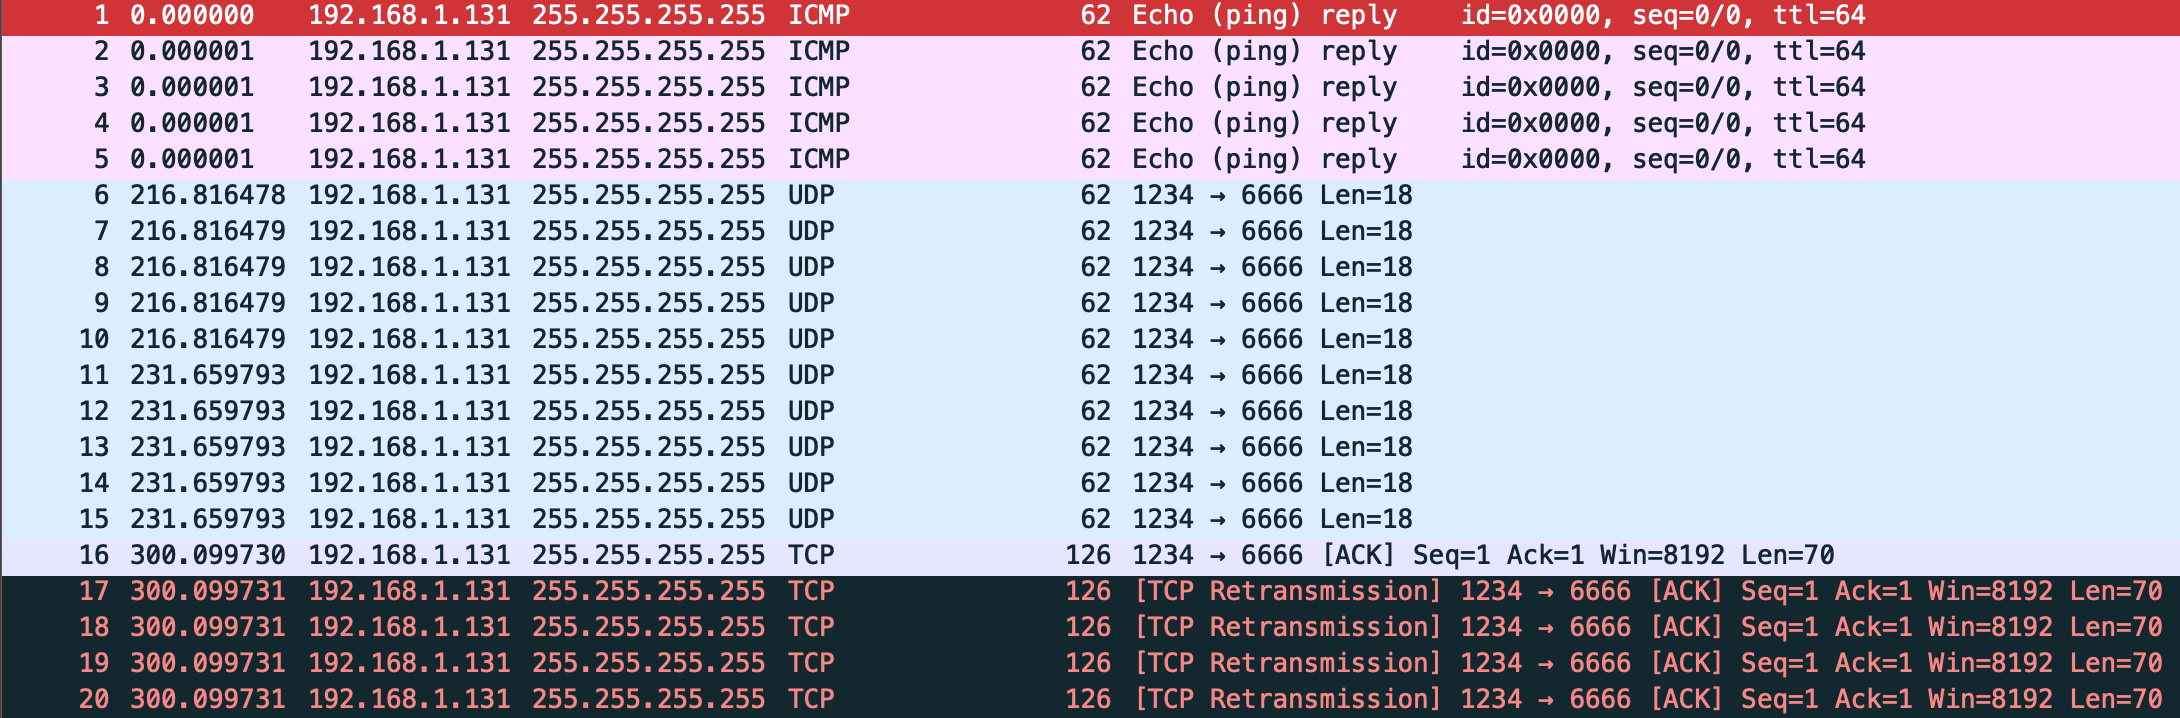
\includegraphics[scale=0.25]{images/wireshark.png} 
\centering
\caption{\textit{Manipolazione dei Pacchetti con Pktgen, analisi con Wireshark}} \cite{noauthor_wireshark_nodate}
\label{fig:wireshark}
\vspace{1cm}
\end{figure}
\FloatBarrier

\FloatBarrier
\begin{figure}[h]
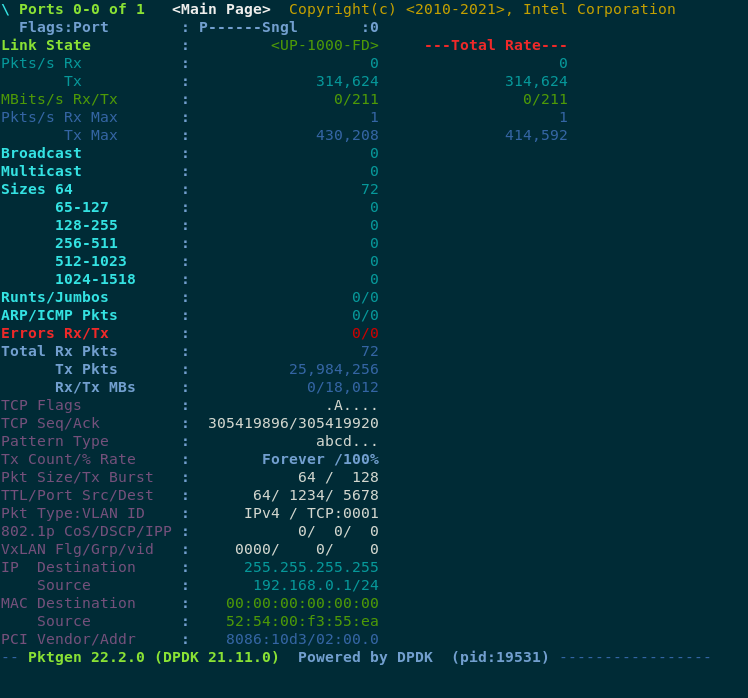
\includegraphics[scale=0.4]{images/pktgen_1.png}
\centering
\caption{\textit{Interfaccia di Pktgen}}
\vspace{1cm}
\label{fig:pktgen_1}
\end{figure}
\FloatBarrier


\section*{Infrastrutture}
\addcontentsline{toc}{subsection}{Infrastrutture}

\subsection*{Test all' interno della stessa Macchina Virtuale}
\addcontentsline{toc}{subsection}{Test all' interno della stessa Macchina Virtuale}
Nell' infrastruttura in \textbf{{Figura \ref{fig:dpdk_vm1}}} il test viene eseguito in una macchina virtuale in cui è presente un unico host, collegato ad una scheda di rete paravirtualizzata. Lo stesso host si mette in ascolto e in ricezione. Sono stati utilizzati in totale 2 core ed il master core.
Il primo core resta in trasmissione (TX) mentre il secondo in ricezione (RX). I due core sono dedicati alla stessa istanza di Pktgen. I test fanno riferimento alla stessa scheda di rete, l'host dispone di 4GB di RAM.
\FloatBarrier
\begin{figure}[h]
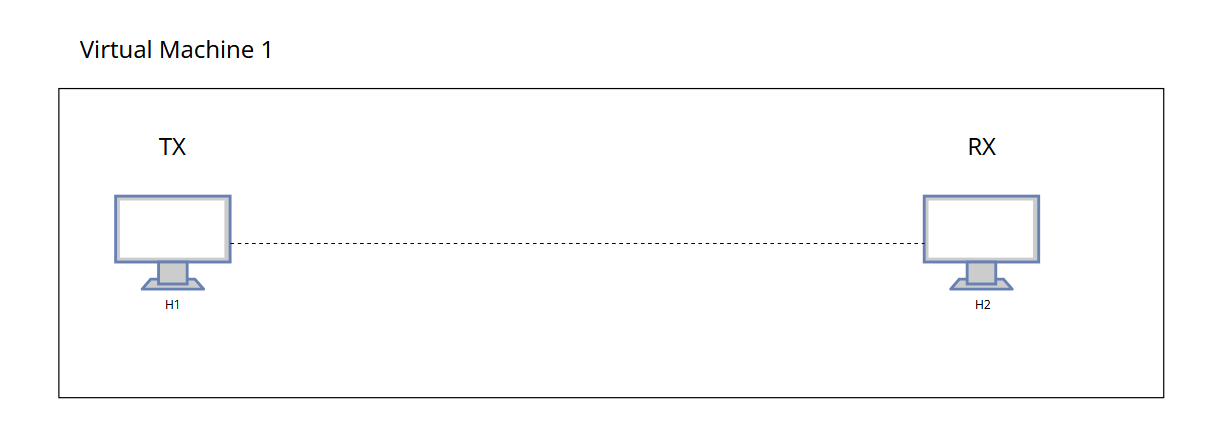
\includegraphics[scale=0.5]{images/dpdk_vm1.png}
\centering
\caption{\textit{Test in macchina virtuale con un unico host}}
\vspace{1cm}
\label{fig:dpdk_vm1}
\end{figure}
\FloatBarrier
\leavevmode\newline
Per configurare le operazioni che deve eseguire il primo core di trasmissione dall'interfaccia di pktgen si può usare la seguente configurazione
\begin{minted}[
frame=lines,
framesep=2mm,
baselinestretch=1.2,
bgcolor=white,
fontsize=\footnotesize,
linenos
]{bash}
set 0 src ip 192.168.100.1/24
set 0 dst ip 192.168.100.1/24
set 0 dst mac 00:00:00:00:00:01
set 0 src mac 00:00:00:00:00:01
set 0 size 64
set 0 pattern user
set 0 user pattern test
\end{minted}

\subsection*{Test tra due Macchine Virtuali}
\addcontentsline{toc}{subsection}{Test tra due Macchine Virtuali}
In \textbf{{Figura \ref{fig:dpdk_vm2}}} il test viene eseguito tra due host in due macchine virtuali collegate in rete interna. I due host sono collegati alla stessa scheda di rete fisica, ma virtualmente a due schede di rete paravirtualizzate con due IP e due indirizzi MAC diversi. H1 è l'host che effettua la trasmissione, mentre H2 effettua la ricezione. Sono stati utilizzati in totale 1 core ed il master core per ogni istanza di Pktgen. Ogni host dispone di 4GB di RAM, per un totale complessivo di 8GB.
\FloatBarrier
\begin{figure}[h]
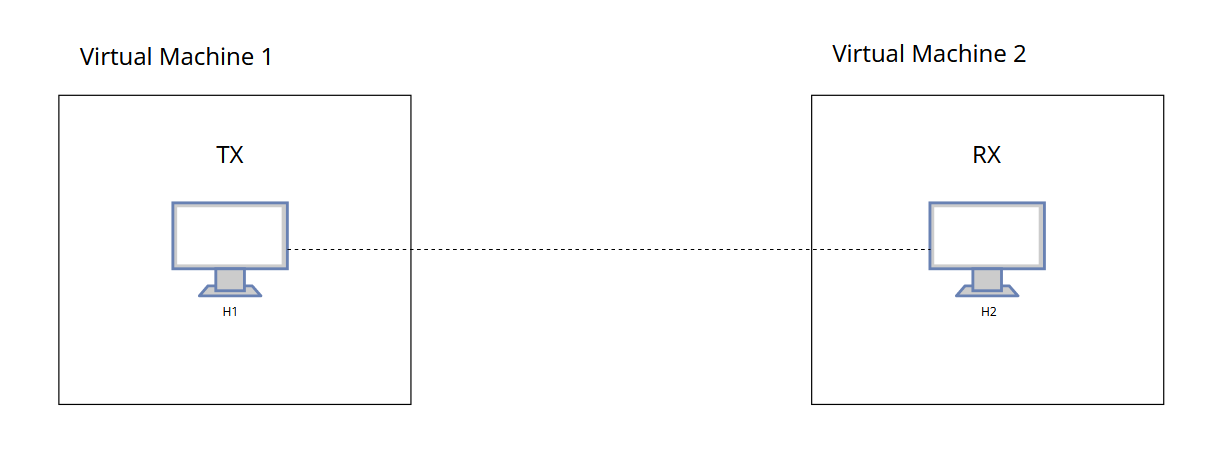
\includegraphics[scale=0.5]{images/dpdk_vm2.png}
\centering
\caption{\textit{Test tra due NIC di due Host in due macchine virtuali}}
\label{fig:dpdk_vm2}
\vspace{1cm}
\end{figure}
\FloatBarrier

In questo caso si specifica l'IP e il MAC del secondo host, in modo da far arrivare i pacchetti a destinazione.
\begin{minted}[
frame=lines,
framesep=2mm,
baselinestretch=1.2,
bgcolor=white,
fontsize=\footnotesize,
linenos
]{bash}
set 0 src ip 192.168.100.1/24
set 0 dst ip 192.168.100.2/24
set 0 dst mac 00:00:00:00:00:01
set 0 src mac 00:00:00:00:00:02
set 0 size 64
set 0 pattern user
set 0 user pattern test
\end{minted}


\subsection*{Test in rete interna in condizioni reali}
\addcontentsline{toc}{subsection}{Test in rete interna in condizioni reali}
La \textbf{{Figura \ref{fig:dpdk_lan2}}} mostra il test effettuato in una rete locale, in cui i due host sono due calcolatori diversi, collegati tra loro da uno switch. In questo caso gli host dispongono di schede di rete fisiche con indirizzi fisici e risiedono all'interno di una rete domestica. H1 è l'host che effettua la trasmissione, mentre H2 effettua la ricezione. Sono stati utilizzati in totale 4 core ed il master core per ogni istanza di Pktgen. Ogni calcolatore dispone di 16GB di RAM.
\FloatBarrier
\begin{figure}[h]
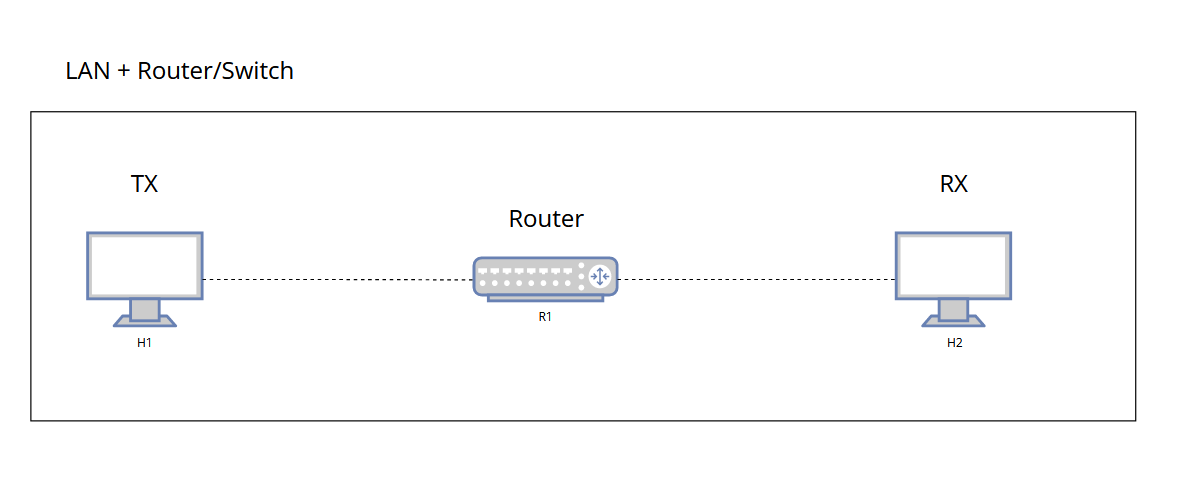
\includegraphics[scale=0.5]{images/dpdk_lan2.png}
\centering
\caption{\textit{Test tra due NIC di due Host nella stessa LAN passando per un Router}}
\vspace{1cm}
\label{fig:dpdk_lan2}
\end{figure}
\FloatBarrier



\begin{minted}[
frame=lines,
framesep=2mm,
baselinestretch=1.2,
bgcolor=white,
fontsize=\footnotesize,
linenos
]{bash}
set 0 src ip 192.168.1.17/24
set 0 dst ip 192.168.1.18/24
set 0 dst mac d8:d3:85:ea:1b:ee
set 0 src mac 00:1b:63:84:45:e6
set 0 size 64
set 0 pattern user
set 0 user pattern test
\end{minted}


\section*{Sviluppo del progetto: P4}
\addcontentsline{toc}{section}{Sviluppo del progetto: P4}

\subsection*{Setup}
\addcontentsline{toc}{subsection}{Setup}
Per creare l'infrastruttura di uno o più switch P4 collegati a due host, si deve per prima cosa disporre di due schede di rete paravirtualizzate. Per avere queste due interfacce di sono stati utilizzati i driver MacVTAP. Una volta create le NIC virtuali, è opportuno creare anche due namespace collegati tramite veth e caricare il programma P4 negli switch. Anche in questa fase di setup ci si è serviti di un software esterno per generare traffico. Questa volta è stato utilizzato IPerf3 \cite{noauthor_iperf_nodate} su protocollo TCP.


\subsection*{Accept e Forward}
\addcontentsline{toc}{subsection}{Accept e Forward}
Il seguente snippet di codice mostra l' Ingress Processing del semplice programma usato per fare Accept e Forward ed è caricato in tutte le configurazioni degli switch \cite{noauthor_p4_2022-1}. La versione utilizzata è P4$_{\mbox{16}}$.
\begin{minted}[
frame=lines,
framesep=2mm,
baselinestretch=1.2,
bgcolor=white,
fontsize=\footnotesize,
linenos
]{c}
control MyIngress(inout headers hdr,
                  inout metadata meta,
                  inout standard_metadata_t standard_metadata) {
    action drop() {
        mark_to_drop(standard_metadata);
    }

    action ipv4_forward(macAddr_t dstAddr, egressSpec_t port) {
        standard_metadata.egress_spec = port;
        hdr.ethernet.srcAddr = hdr.ethernet.dstAddr;
        hdr.ethernet.dstAddr = dstAddr;
        hdr.ipv4.ttl = hdr.ipv4.ttl - 1;
    }

    table ipv4_lpm {
        key = {
            hdr.ipv4.dstAddr: lpm;
        }
        actions = {
            ipv4_forward;
            drop;
            NoAction;
        }
        size = 1024;
        default_action = drop();
    }

    apply {
        if (hdr.ipv4.isValid()) {
            ipv4_lpm.apply();
        }
    }
}
\end{minted}
Le regole di forward saranno aggiunte nei singoli switch in successiva fase di runtime.
\pagebreak

\subsection*{Test di trasmissione tra due host con uno switch P4}
\addcontentsline{toc}{subsection}{Test di trasmissione tra due host con uno switch P4}

Nell'infrastruttura mostrata in \textbf{{Figura \ref{fig:p4_basic}}} si hanno due host collegati tra di loro passanti per uno switch P4.
\FloatBarrier
\begin{figure}[h]
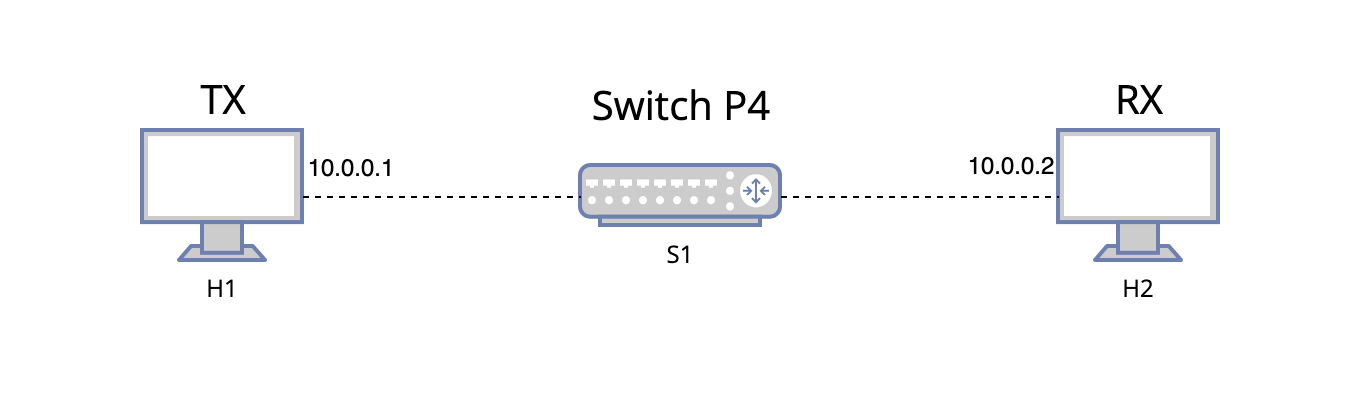
\includegraphics[scale=0.5]{images/p4_basic.png}
\centering
\caption{\textit{Test tra due host passando per uno switch P4}}
\label{fig:p4_basic}
\vspace{1cm}
\end{figure}
\FloatBarrier
\leavevmode\newline
Per avviare il singolo switch si può usare
\begin{minted}[
frame=lines,
framesep=2mm,
baselinestretch=1.2,
bgcolor=white,
fontsize=\footnotesize,
linenos
]{bash}
sudo ./simple_switch -i 1@s1-eth0 -i 2@s1-eth1 basic.json
--thrift-port 9091 --notifications-addr ipc:///tmp/bmv2-1-notifications.ipc
\end{minted}
E poi a runtime per caricare le regole 

\begin{minted}[
frame=lines,
framesep=2mm,
baselinestretch=1.2,
bgcolor=white,
fontsize=\footnotesize,
linenos
]{bash}
table_clear MyIngress.ipv4_lpm
table_add MyIngress.ipv4_lpm MyIngress.ipv4_forward 10.0.0.1/32 => 00:00:00:00:00:01 1
table_add MyIngress.ipv4_lpm MyIngress.ipv4_forward 10.0.0.2/32 => 00:00:00:00:00:01 2
\end{minted}

\subsection*{Test di trasmissione tra due host con due switch P4}
\addcontentsline{toc}{subsection}{Test di trasmissione tra due host con due switch P4}
Nello scenario in \textbf{{Figura \ref{fig:p4_double}}} sono invece presenti due host collegati tra di loro e passanti per due switch P4. Le configurazioni si duplicano rispetto al caso precedente.

\FloatBarrier
\begin{figure}[h]
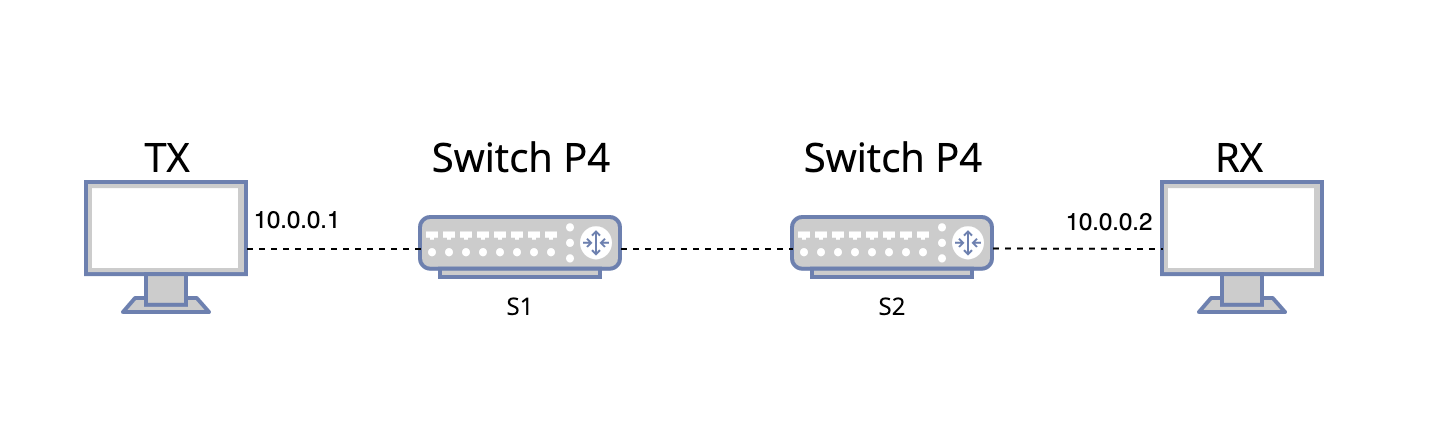
\includegraphics[scale=0.5]{images/p4_double.png}
\centering
\caption{\textit{Test tra due host passando per due switch P4}}
\label{fig:p4_double}
\vspace{1cm}
\end{figure}
\FloatBarrier
\leavevmode\newline
Per caricare le regole sui due switch utilizziamo
\begin{minted}[
frame=lines,
framesep=2mm,
baselinestretch=1.2,
bgcolor=white,
fontsize=\footnotesize,
linenos
]{bash}
sudo ./simple_switch -i 1@s1-eth0 -i 2@s1-eth1 basic.json
--thrift-port 9091 --notifications-addr ipc:///tmp/bmv2-1-notifications.ipc
sudo ./simple_switch -i 1@s2-eth0 -i 2@s2-eth1 basic.json 
--thrift-port 9092 --notifications-addr ipc:///tmp/bmv2-2-notifications.ipc
\end{minted}
La configurazione a runtime diventa la seguente 
\subsubsection*{Switch S1}
\begin{minted}[
frame=lines,
framesep=2mm,
baselinestretch=1.2,
bgcolor=white,
fontsize=\footnotesize,
linenos
]{bash}
table_clear MyIngress.ipv4_lpm
table_add MyIngress.ipv4_lpm MyIngress.ipv4_forward 10.0.0.1/32 => 00:00:00:00:00:01 1
table_add MyIngress.ipv4_lpm MyIngress.ipv4_forward 10.0.0.2/32 => 00:00:00:00:00:02 2
\end{minted}
\subsubsection*{Switch S2}
\begin{minted}[
frame=lines,
framesep=2mm,
baselinestretch=1.2,
bgcolor=white,
fontsize=\footnotesize,
linenos
]{bash}
table_clear MyIngress.ipv4_lpm
table_add MyIngress.ipv4_lpm MyIngress.ipv4_forward 10.0.0.2/32 => 00:00:00:00:00:03 1
table_add MyIngress.ipv4_lpm MyIngress.ipv4_forward 10.0.0.1/32 => 00:00:00:00:00:04 2
\end{minted}
\newpage
\chapter*{Capitolo 4}
\addcontentsline{toc}{chapter}{Capitolo 4}


\section*{Risultati}
\addcontentsline{toc}{section}{Risultati}


\section*{DPDK}
\addcontentsline{toc}{section}{DPDK}
I Test con DPDK hanno riportato i seguenti risultati.
I risultati di ricezione e trasmissione virtuale riguardano l'effettivo throughput generabile da DPDK, ovvero la capacità limite di generazione e ricezione di pacchetti che si ha per la specifica infrastruttura.
I risultati di ricezione reale invece indicano la quantità di dati effettivamente ricevuti dalla scheda di rete e registrati con il programma \textbf{bwm-ng} \cite{noauthor_bwmng} sul computer host. Appare chiaro che disponendo di una scheda di rete Gigabit è impossibile ricevere un flusso di dati superiore a questo valore.
Parte dei test in macchina virtuale sono stati eseguiti anche attivando il PCI Passthrough, ma i risultati riportati si discostano di pochi Mbit/s dai test con le interfacce MacVTap e quindi non sono riportati. Questo distaccamento minimo è possibile grazie alla grande efficienza dei driver MacVTap in combinazione con il Kernel Bypassing effettuato da DPDK.

\vspace{1cm}
\begin{center}
\begin{tabular}[h!]{ |c|c|c|c|c| } 
\hline
\rule{0pt}{4ex}
Infrastruttura & Trasmissione virtuali & Ricezione virtuali & Trasmissione effettivi & Ricezione effettivi \\
\hline
\rule{0pt}{4ex}
\textbf{{Figura \ref{fig:dpdk_vm1}}} & 800Mbit/s & 800Mbit/s & 800Mbit/s & 800Mbit/s \\ 
\hline
\rule{0pt}{4ex}
\textbf{{Figura \ref{fig:dpdk_vm2}}}& 3Gbit/s & 3Gbit/s & 1Gbit/s & 1Gbit/s\\ 
\hline
\rule{0pt}{4ex}
\textbf{{Figura \ref{fig:dpdk_lan2}}} & 10Gbit/s & 1Gbit/s & 1Gbit/s & 1Gbit/s\\
\hline
\end{tabular}
\end{center}
\vspace{1cm}

\label{fig:dpdk_differences}

\subsection*{Considerazioni}
\addcontentsline{toc}{subsection}{Considerazioni}
\leavevmode\newline
Nei test mostrati in \textbf{{Figura \ref{fig:dpdk_vm1}}}
 la velocità di trasmissione è ridotta rispetto ai test successivi perché DPDK è CPU intensive. In questo caso infatti sullo stesso host ci sono due istanze running di DPDK, una per l'invio e una per la ricezione dei pacchetti che, secondo la semantica dei Poll Mode Drivers, chiedono in modalità polling alla CPU la presenza di pacchetti da processare.
\leavevmode\newline
\\
In \textbf{{Figura \ref{fig:dpdk_vm2}}} invece i test presentano un risultato migliore in termini di performance a livello Data Plane: in questo caso gli interrupt generati dai Poll Mode Drivers sono su due processori diversi in due macchine virtuali diverse risultando in una gestione generalmente migliore. In questo caso, inoltre, ogni macchina virtuale ha due core dedicati, in contrapposizione al precedente caso di singola macchina virtuale con due core totali.
\leavevmode\newline
\\
Nei test in \textbf{{Figura \ref{fig:dpdk_lan2}}} siamo in condizioni reali, ovvero in una rete domestica con un router che si occupa di amministrare i pacchetti spediti dal dispositivo con DPDK. In questo caso, disponendo di una grande capacità di calcolo, ovvero con 4 core dedicati alla generazione dei pacchetti, è possibile riuscire a generare fino a 10 Gbit/s. Non è possibile far passare tale quantità di dati al secondo attraverso il router a causa del limite fisico della scheda di rete. L'invio dei pacchetti infatti sarà limitato alla capacità massima di invio di 1Gbit/s tipico delle NIC standard. Anche se la scheda di rete fosse capace di generare un tale bitrate, il router genererebbe ``bottleneck", disponendo anch'esso di porte Gigabit Ethernet.
La ricezione virtuale e fisica in questo caso, quindi, coincideranno.

\subsection*{Problematiche}
\addcontentsline{toc}{subsection}{Problematiche}
Durante il testing di DPDK, uno dei problemi maggiori è stato monitorare l'invio dei pacchetti senza il tool Pktgen. Sfruttando il Kernel Bypass, DPDK si stacca completamente dal Kernel e si astrae nello user-space, quindi è praticamente impossibile riuscire a leggere i pacchetti in ricezione e in trasmissione se non con dei programmi che sfruttano le librerie apposite di DPDK in user-space. Nei test in macchina virtuale è stato però comunque possibile riuscire a leggere il traffico che DPDK generava, leggendo il buffer delle interfacce MacVTap, potendo monitorare l'effettivo throughput anche da una fonte esterna a Pktgen.


\section*{P4}
\addcontentsline{toc}{section}{P4}

I test con P4 hanno riportato i seguenti risultati.
In questo tipo di setup i test sono stati eseguiti solo in una rete interna tra macchine virtuali, quindi non è presente la distinzione tra throughput effettivo e virtuale. Ogni switch riceve i pacchetti, li accetta e li inoltra se l'header fa match con l'header ethernet o l'header IPv4.

\vspace{1cm}
\begin{center}
\begin{tabular}[h!]{ |c|c|c| } 
\hline
\rule{0pt}{4ex}
Infrastruttura & Trasmissione & Ricezione \\
\hline
\rule{0pt}{4ex}
\textbf{{Figura \ref{fig:p4_basic}}} & 830Mbit/s & 830Mbit/s \\ 
\hline
\rule{0pt}{4ex}
\textbf{{Figura \ref{fig:p4_double}}} & 425Mbit/s & 425Mbit/s \\ 
\hline
\end{tabular}
\end{center}
\vspace{1cm}

\FloatBarrier
\begin{figure}%
    \centering
    \subfloat[\centering H1]{{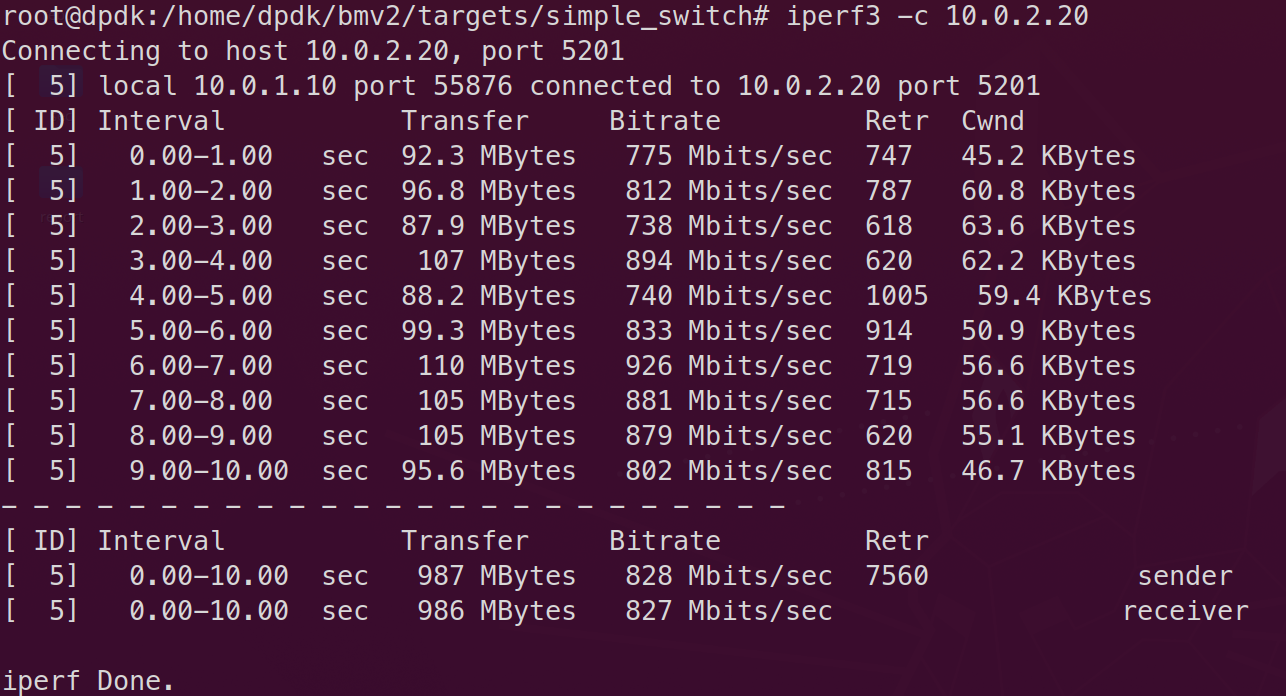
\includegraphics[width=7.5cm]{images/h1_p4basic_patrick.png} }}%
    \qquad
    \subfloat[\centering H2]{{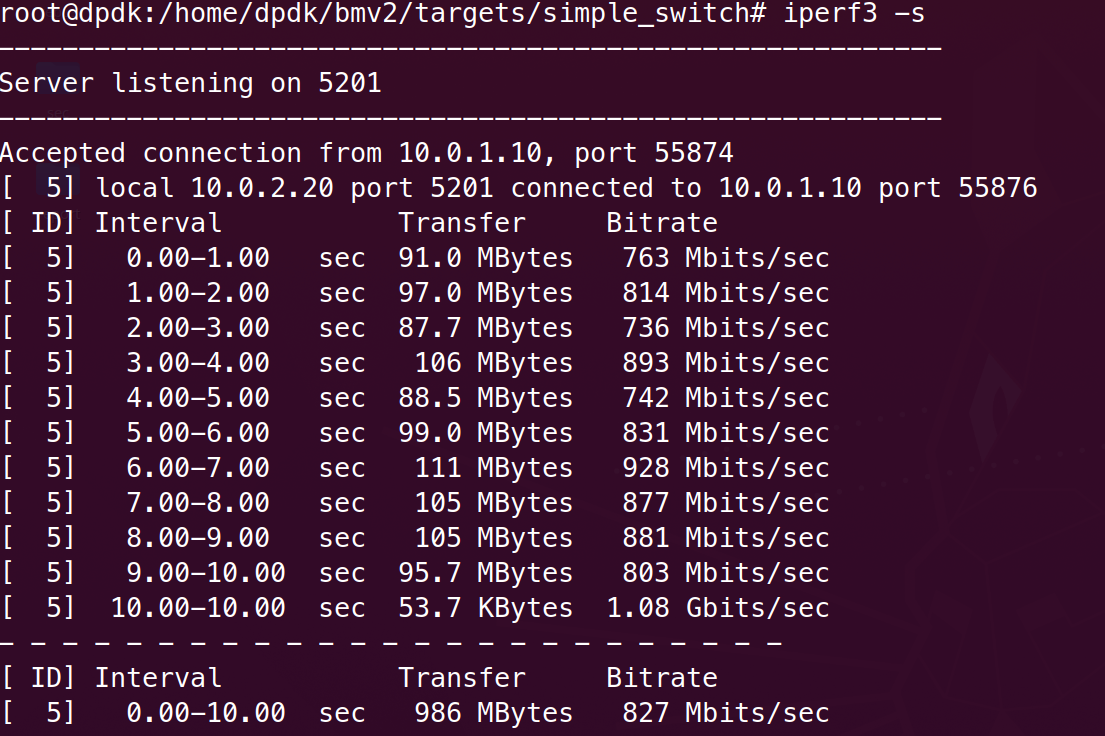
\includegraphics[width=7cm]{images/h2_p4basic_patrick.png} }}%
    \caption{P4 single switch}%
    \label{fig:h1_p4basic_patrick}%
\end{figure}
\FloatBarrier


\FloatBarrier
\begin{figure}%
    \centering
    \subfloat[\centering H1]{{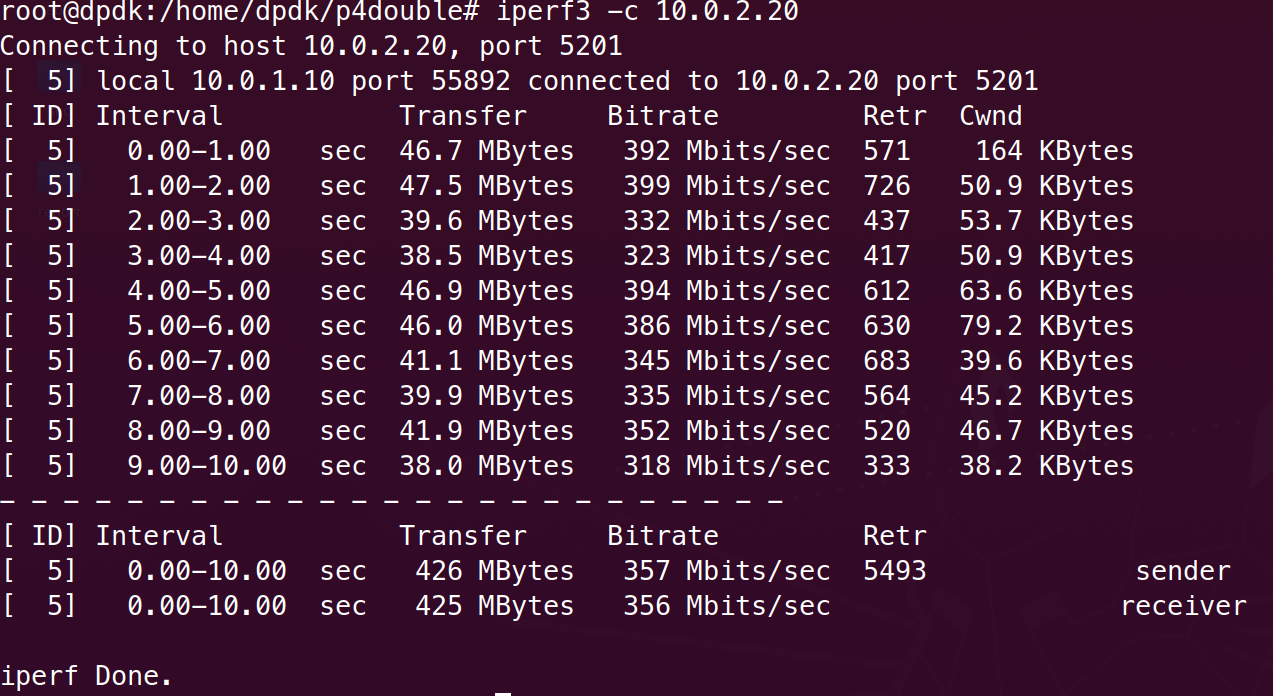
\includegraphics[width=7.5cm]{images/h1_p4double_patrick.png} }}%
    \qquad
    \subfloat[\centering H2]{{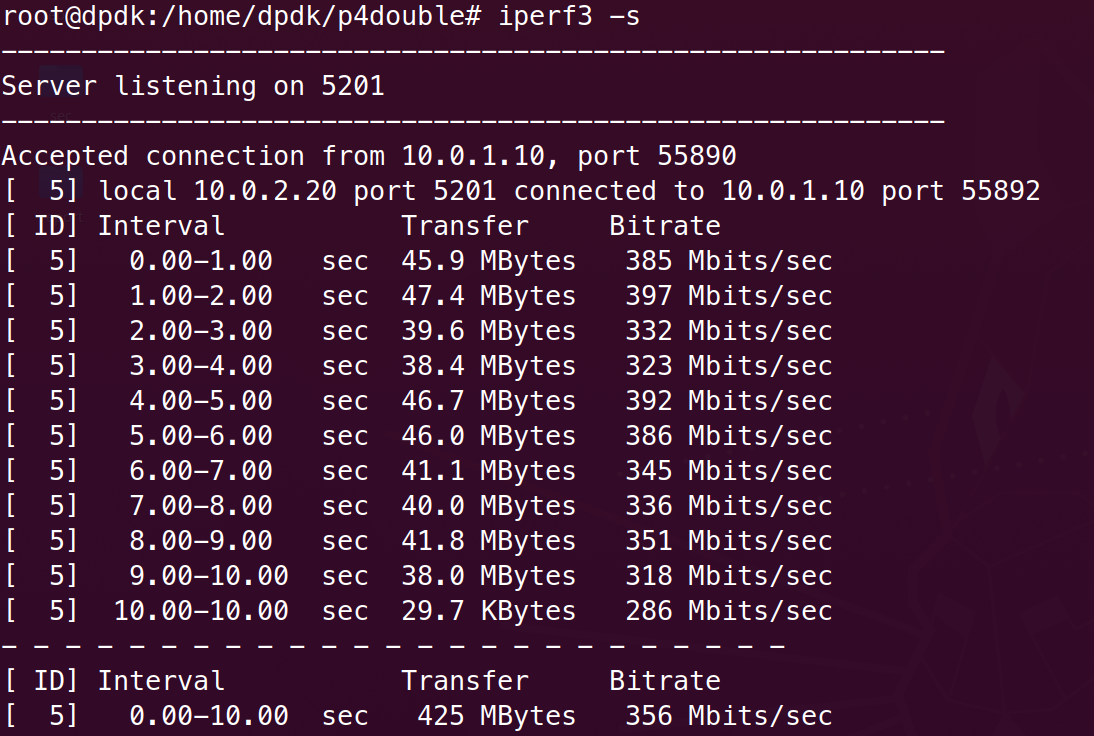
\includegraphics[width=7cm]{images/h2_p4double_patrick.png} }}%
    \caption{P4 double switch}%
    \label{fig:h1_p4double_patrick}%
\end{figure}
\FloatBarrier

\subsection*{Considerazioni}
\addcontentsline{toc}{subsection}{Considerazioni}
I test in \textbf{{Figura \ref{fig:h1_p4basic_patrick}}}
 mostrano le prestazioni di un semplice forwarding. Le prestazioni sono poco sotto il Gigabit in TX (\textbf{{Figura \ref{fig:h1_p4basic_patrick}.a}}) e in RX (\textbf{{Figura \ref{fig:h1_p4basic_patrick}.b}}) perché in condizioni ideali su un host reale non virtualizzato, BMv2 ha un throughput medio di 1047 Mbit/s \cite{noauthor_behavioral_2022}. È quindi ordinario aver un basso bitrate a causa del target su cui si esegue il programma P4, che è infatti solo a scopo di test. 
\leavevmode\newline
\\
Nei test in \textbf{{Figura \ref{fig:h1_p4double_patrick}}} si sottolinea come le prestazioni calano significativamente aggiungendo in cascata un ulteriore switch. In \textbf{{Figura \ref{fig:h1_p4double_patrick}.a}} sono presenti i test di trasmissione, in \textbf{{Figura \ref{fig:h1_p4double_patrick}.b}} sono presenti i test in ricezione.
\leavevmode\newline
\\
Il target BMv2 può avere scarse prestazioni per diversi motivi, alcuni dei quali possono essere i seguenti
\begin{itemize}
    \item Performance dell'hardware sottostante
    \item La complessità del programma P4 caricato: all'aumento della complessità del programma segue l'aumento della latenza
    \item Il compilatore utilizzato per generare il JSON
    \item Utilizzo in macchina virtuale
\end{itemize}
\subsection*{Problematiche}
\addcontentsline{toc}{subsection}{Problematiche}
Durante il setup dell'ambiente, dopo aver testato il ping tra i namespace H1 e H2, si può procedere testando le prestazioni con il software IPerf3 \cite{noauthor_iperf_nodate}. Durante questa fase è stato difficile capire perché i dispositivi non riuscissero a stabilire una connessione sfruttando questo tool. Uno dei motivi possibili per spiegare questo evento è che durante il tragitto attraverso gli switch, il parser e il deparser di BMv2 andassero a modificare il checksum degli header IPv4. Per risolvere il problema è possibile disabilitare il \textbf{TCP checksum offloading}, che serve per controllare la validità del checksum degli header.
È possibile disabilitare tale funzionalità su entrambi gli host attraverso il seguente comando, utilizzando ethtool \cite{noauthor_ethtool8_nodate}. In questo modo è possibile sfruttare IPerf3 con il protocollo TCP \cite{noauthor_cant_nodate}.
\begin{minted}{bash}
ethtool -K ethX rx off tx off
\end{minted}
\pagebreak
\section*{Punti aperti e sviluppi futuri}
\addcontentsline{toc}{section}{Punti aperti e sviluppi futuri}

\addcontentsline{toc}{subsection}{P4Pi}
\subsection*{P4Pi}
In futuro sarebbe interessante studiare tecnologie e altri target P4. Un progetto di nome P4Pi \cite{noauthor_getting_2022} porta la compatibilità di P4 sui Raspberry Pi, dei Single Board Computer economici. Così facendo sarebbe possibile agganciare in modo ``Plug and Play" a delle reti questi dispositivi così da poterli utilizzare come switch o router.\\

\addcontentsline{toc}{subsection}{OVS-P4}
\subsection*{OVS-P4}
Un altro progetto che estende le funzionalità di P4 è OVS-P4 \cite{osinski_p4-ovs_2022}. Lo scopo di questa estensione di P4 è quella di incrementare le prestazioni degli switch P4 tramite OpenVSwtich sfruttando tecnologie come uBPF \cite{noauthor_ubpf} e DPDK.
Questo è possibile perché la modifica a livello di Data Plane appare trasparente a OVS che continua a comportarsi come switch ma con prestazioni di inoltro maggiori.
OVS, come nella sua versione standard, può implementare DPDK, beneficiando dei vantaggi di forwarding che questo framework offre. Sfruttando DPDK non è più necessario separare user-space e Kernel, ma è possibile implementare accanto allo switch virtuale i metodi di Kernel Bypassing. In questo modo si completano in user-space Data Plane e Control Plane, così da avere un bypass completo del Kernel. \\
OVS sfrutta così DPDK ma mantiene anche la versatilità offerta dai programmi P4 applicati ai virtual switch di cui dispone.
In \textbf{{Figura \ref{fig:ovs_dpdk}}}
 si notano le differenze tra l'utilizzo di OVS con e senza DPDK.
\vspace{2cm}
\FloatBarrier
\begin{figure}[h]
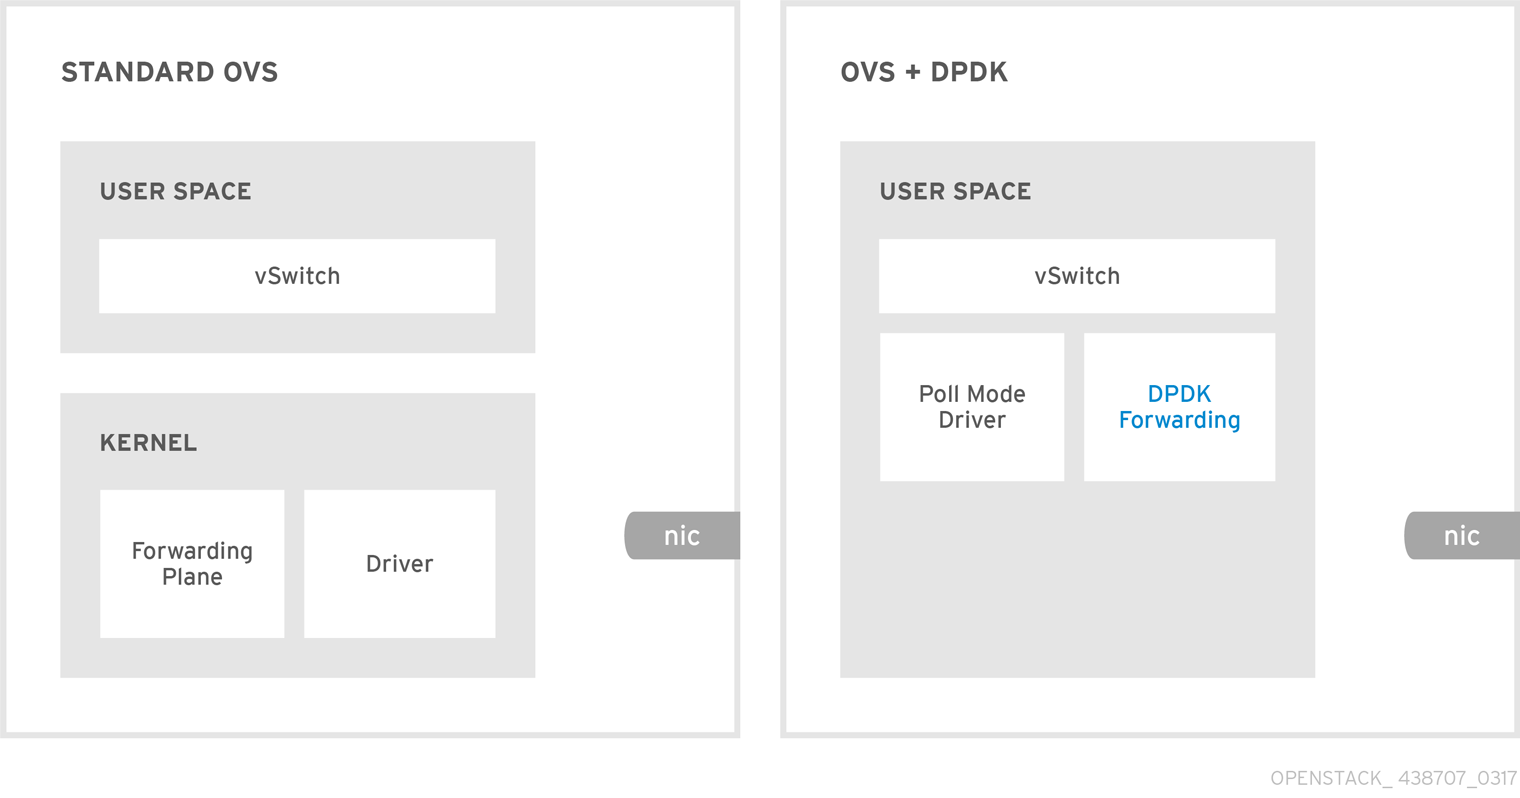
\includegraphics[scale=0.27]{images/ovs_dpdk.png}
\centering
\caption{\textit{OVS and OVS with DPDK}}
\label{fig:ovs_dpdk}
\end{figure}
\FloatBarrier

\addcontentsline{toc}{subsection}{T4P4S}
\subsection*{T4P4S}
T4P4S (Translator for P4 Switches) è un progetto che ha lo scopo di generare codice P4 ad alte prestazioni \cite{noauthor_p4elte_nodate}. Il compilatore P4 genera un file JSON, T4P4S esegue il parsing e genera codice C che viene poi collegato alle API di DPDK. Questo compilatore sfruttando le API generiche di C riesce a garantire prestazioni elevate, arrivando a superare le prestazioni di OVS+DPDK nei benchmark di forwarding, quindi a puro livello di Data Plane.
In \textbf{{Figura \ref{fig:t4p4s}}} si nota la pipeline di compilazione di un programma P4 in codice C per lo specifico target.
\FloatBarrier
\vspace{1cm}
\begin{figure}[h]
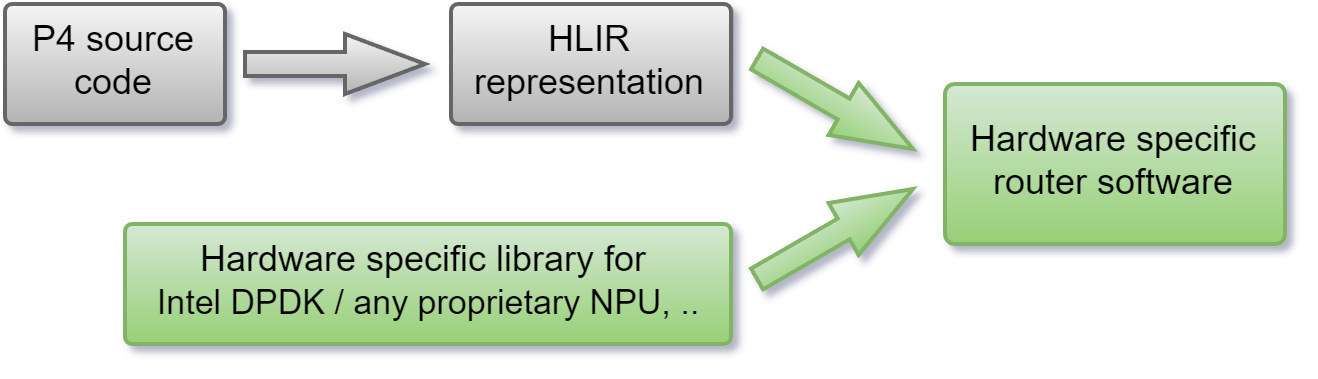
\includegraphics[scale=0.40]{images/t4p4s.png}
\centering
\caption{\textit{T4P4S Compiler}}
\label{fig:t4p4s}
\end{figure}
\FloatBarrier
\leavevmode\newline
La compilazione segue un modello a pipeline. Si inizia da una rappresentazione intermedia (Intermediate Rapresentation) che sarà poi compilata in codice C grazie alle API del Network Hardware Abstraction Layer. È il Core Compiler che si occuperà di generare il codice per lo specifico target, sfruttando le NetHAL API calls. Il Core di T4P4S implementa infatti il ``Packet Parsing" e le ``Actions" di P4 e traduce il tutto in funzioni C.

\pagebreak

\section*{Ambiente di Test}
\addcontentsline{toc}{section}{Ambiente di Test}

\subsection*{Computer Host}
\addcontentsline{toc}{subsection}{Computer Host}
La macchina host su cui sono stati eseguiti i test e su cui sono state lanciate le macchine virtuali dispone dei seguenti requisiti hardware

\begin{itemize}
    \item CPU: I5 6600K 4 Core 4 Thread 64 Bit
    \item RAM: 16 GB 2900MHz
    \item S.O: Linux Ubuntu 20.04 LTS
    \item NIC: Intel Ethernet 1219-V full duplex 1GBit/s
\end{itemize}

\subsection*{Virtual Machine}
\addcontentsline{toc}{subsection}{Virtual Machine}
Le Virtual Machine sono copie di una singola macchina virtuale con le seguenti specifiche
\begin{itemize}
    \item CPU: 2 Cores
    \item RAM: 4GB
    \item S.O: Linux Ubuntu 20.04 LTS
    \item HDD: 50GB
\end{itemize}

\subsection*{Virtualizzazione}
\addcontentsline{toc}{subsection}{Virtualizzazione}
\begin{itemize}
    \item Software di Virtualizzazione: QEMU/KVM \cite{noauthor_qemu_nodate}
    \item Paravirtualized drivers: VirtIO
    \item Device Drivers: MacVTap
\end{itemize}




\newpage
\chapter*{Capitolo 5}
\addcontentsline{toc}{chapter}{Capitolo 5}

\section*{Conclusioni}
\addcontentsline{toc}{section}{Conclusioni}


In un futuro in cui è sempre più cruciale la velocità di connessione tra dispositivi e sono più presenti l' Internet of Things e il Cloud Computing, le SDN si collocano come potenziale punto di unione tra le necessità delle nuove tecnologie e la forza di avere un networking volto all' open source. Con il paradigma della rete aperta e programmabile si possono introdurre innovazioni a livello Data Plane e Control Plane.\\
\newline 
Lo scopo della tesi è stato quello di analizzare le prestazioni grezze e le potenzialità di DPDK, cercando di unire la velocità del forwarding di quest'ultimo alla versatilità, quindi programmabilità, del piano di controllo gestito da uno switch P4. 
L'analisi delle prestazioni di DPDK fa risaltare la potenza della tecnologia, che sfruttando il Kernel Bypassing, è capace di generare un traffico molto elevato anche disponendo di hardware a basse prestazioni. I test sono stati eseguiti trasmettendo pacchetti da 1500 byte, così da ottenere una quantità maggiore di dati trasmessi.\\
\newline
I risultati in condizioni reali riportano un throughput medio di 10 Gbit/s che per le reti odierne è sicuramente un risultato interessante, avendo la capacità di gestire in media qualche giga di dati. 
Le librerie di DPDK sono generalmente pensate per agire su di un flusso di dati suddiviso in pacchetti di piccola dimensione (64 byte). Negli usi applicativi moderni, come ad esempio scenari di streaming o flussi dati costanti, è difficile riuscire a segmentare il traffico in pacchetti di così piccola taglia.
Un ulteriore limite di DPDK può essere trovato nell' usabilità di questo framework. Nella fase di test è stato utilizzato un tool in grado di generare una enorme quantità di pacchetti per valutare le performance di instradamento. Dal punto di vista dell' utilizzo, sarebbe utile usufruire di questa tecnologia in modo trasparente, ovvero poter delegare alla scheda di rete le operazioni quotidiane senza accorgersi del livello sottostante e rendere così compatibile DPDK con il livello applicativo, come ad esempio la navigazione su Internet o l'invio di file ad altri dispositivi.\\
\newline
P4 ha dimostrato grande potenzialità grazie alla sua riprogrammabilità e DPDK si è confermato un'ottima tecnologia per velocizzare il forwarding di pacchetti. 
Coniugando P4 e DPDK sarebbe possibile unire la versatilità che ha uno switch P4 con il suo approccio ``top-down", alla velocità di instradamento dei dati che offre DPDK anche con un hardware mediocre. Un approccio molto interessante si è rivelato quello del progretto P4-OVS. In questa estensione di OVS, è possibile ottenere prestazioni elevate, in modo da rimpiazzare lo standard Kernel Datapath di cui dispone, con un Datapath completamente basato su DPDK \cite{noauthor_p4ovs}. Nella pratica l'uso di OpenVSwitch resta lo stesso a livello di networking, ma eredita i benefici del packet processing che porta P4 e del forwarding interno di pacchetti che è accelerato grazie al driver DPDK ad alte prestazioni. 

\chapter*{Ringraziamenti}
\addcontentsline{toc}{chapter}{Ringraziamenti}
Ringrazio i relatori ed il team di \href{https://ulisse.unibo.it/}{ULISSe} per avermi dato l'opportunità di lavorare su questo tema di ricerca.\\
\newline
Vorrei inoltre ringraziare e dedicare questa tesi alla mia famiglia e alle mie persone speciali.

\newpage
\myemptypage

\printbibliography
\listoffigures

\newpage
\end{document}
